\documentclass[11pt]{article}

% ---------- page geometry ----------
\usepackage[a4paper,top=2.1cm,bottom=2.1cm,left=2.2cm,right=2.2cm]{geometry}
\setlength{\emergencystretch}{2em}

% ---------- fonts: Times for text and mathematics ----------
\usepackage{fontspec}
\setmainfont{TeX Gyre Termes}[Ligatures=TeX]
\usepackage{unicode-math}
\setmathfont{TeX Gyre Termes Math}

% ---------- mathematics ----------
\usepackage{amsmath}
\usepackage{mathtools}

% ---------- tables and figures ----------
\usepackage{booktabs}
\usepackage{multirow}
\usepackage{graphicx}
\usepackage{caption}
\captionsetup{font=small,labelfont=bf,skip=2pt}
\usepackage{subcaption}

% ---------- colour, links, headers ----------
\usepackage{xcolor}
\definecolor{navy}{HTML}{1F3864}
\usepackage[colorlinks=true,linkcolor=navy,citecolor=navy,urlcolor=navy]{hyperref}
\hypersetup{pdftitle={The Geometry of a Bicycle City: Behaviour, Rebalancing, Incentives and Fences in Beijing's Dockless Bike-Share System},
            pdfsubject={2026 CQU MCM Problem C}}
\usepackage{fancyhdr}
\pagestyle{fancy}
\fancyhf{}
\fancyfoot[C]{\thepage}
\renewcommand{\headrulewidth}{0pt}
\usepackage{enumitem}
\usepackage{titlesec}
\titlespacing*{\section}{0pt}{7pt plus 2pt minus 2pt}{3pt}
\titlespacing*{\subsection}{0pt}{6pt plus 1pt minus 1pt}{2pt}
\setlist{itemsep=0pt,topsep=1pt,parsep=0pt}
\usepackage{float}
\renewcommand{\arraystretch}{0.96}
\renewcommand{\topfraction}{0.92}
\renewcommand{\bottomfraction}{0.85}
\renewcommand{\textfraction}{0.06}
\renewcommand{\floatpagefraction}{0.75}
\setcounter{topnumber}{3}
\setcounter{bottomnumber}{3}
\setlength{\textfloatsep}{5pt plus 2pt minus 1pt}
\setlength{\floatsep}{4pt plus 1pt minus 1pt}
\setlength{\intextsep}{4pt plus 1pt minus 1pt}


% ---------- notation shortcuts ----------
\newcommand{\dd}{\mathrm{d}}
\newcommand{\E}{\mathbb{E}}
\newcommand{\Prob}{\mathbb{P}}
\newcommand{\ind}[1]{\mathbb{1}\!\left[#1\right]}
\newcommand{\figref}[1]{Fig.~\ref{#1}}
\newcommand{\tabref}[1]{Table~\ref{#1}}
\newcommand{\eqnref}[1]{Eq.~\eqref{#1}}
\setlength{\parskip}{0pt}
\setlength{\parindent}{0pt}
\setlength{\abovedisplayskip}{3pt}
\setlength{\belowdisplayskip}{3pt}
\setlength{\abovedisplayshortskip}{1pt}
\setlength{\belowdisplayshortskip}{1pt}
\setcounter{tocdepth}{1}

\begin{document}

\thispagestyle{empty}
% ============================ SUMMARY SHEET ============================
\begin{center}
{\Large\bfseries The Geometry of a Bicycle City: Behaviour, Rebalancing,\\ Incentives and Fences in Beijing's Dockless Bike-Share System}\\[6pt]
{\large 2026 CQU Mathematical Contest in Modeling, Problem C}\\[10pt]
\begin{tabular}{ll}
\textbf{Team Control Number:} & \rule{3.2cm}{0.4pt} \\
\textbf{Problem Chosen:} & C \\
\end{tabular}
\end{center}

\vspace{4pt}
\hrule
\vspace{8pt}

\begin{center}{\large\bfseries Summary}\end{center}

Beijing's dockless bike-share system in May 2017 was not short of bicycles. It was
short of bicycles \emph{in the right place at the right time}, and it did not know it.
Using 3.21 million order records from 484,754 bicycles ridden by 349,241 users over
fourteen days, this paper builds one behavioural model and uses it to answer four
operational questions on a common footing.

\textbf{The central finding is a diagnosis of oversupply.} We estimate the fleet at
3.4$\times10^5$ bicycles serving 6.2 rides each per day --- a supply level at which
the daily deficit appears as idle stock rather than unmet demand. At every
resolution we examine, from 50 traffic zones down to 5,263 neighbourhood cells, no
zone ever runs out of bicycles. Every subsequent question is therefore posed as a
question of \emph{cost and placement}, not of shortage.

\textbf{Behaviour (Q1).} Trips are modelled as a marked spatio-temporal point
process: a non-homogeneous Poisson arrival stream, a singly-constrained gravity
destination choice with a time-varying distance-decay parameter, and a
speed-based duration model. The decay parameter is identified by maximum
likelihood and ranges from 2.01 (morning, longer commute trips) to 2.52 (midday,
short errands). On two held-out days the model attains a per-trip log-loss of
3.24--3.52 against 3.28--3.65 for a distance-only benchmark and 7.9--8.2 for an
attraction-only one, and it predicts the top-five destinations correctly 40--48\%
of the time. A latent-class analysis separates five user types whose trip shares
(51.8\% for the multi-purpose majority, 29.6\% for a heavy short-trip minority)
explain the shape of the hourly profile.

\textbf{Rebalancing (Q2).} A time-space network linear program moves bicycles
between 50 zones with a fleet of trucks. Because no zone is ever dry, the binding
constraint is not service but the cost of returning the system to a balanced state:
the optimal plan moves 23,959 bicycles per day (1.12\% of all trips) over 5,441
truck-kilometres, at 3.48 CNY per bicycle relocated. Because the trucks run at
night, the plan is best read as an overnight reset. Rebalancing and fleet size are
substitutes: shrinking the fleet to 80\% of its observed size while adding trucks
lowers total daily cost from 427k to 390k CNY, an interior optimum.

\textbf{Incentives (Q3).} We derive the supply curve of voluntary relocations from
a logit acceptance model in which users trade a cash reward against a detour. The
platform should offer a uniform reward of 1.20 CNY, buying 115,385 relocations
(53.3\% of the peak-hour deficit) for 138k CNY and leaving the rest to trucks --- a
34.9\% saving over moving every bicycle by truck. The limit is physical, not
financial: within a 450 m detour only 71.9\% of the deficit has any qualifying
trip nearby, and reaching 95\% requires a 1,025 m catchment.

\textbf{E-fences (Q4).} Parking demand is the arrival process, whose peak we
characterise by Monte Carlo. A greedy maximal-coverage layout of 626 fences at a
450 m walking radius covers 75.3\% of arrivals; the required capacity is brutally
skewed, with a median of 417 slots and a maximum of 4,827. Electronic fences
without enforced caps merely formalise the bicycle mountain.

\textbf{Competition (Q5).} Splitting the fleet among competing platforms does not
reduce availability in a saturated system --- we verify this down to a 35\% share ---
but it multiplies capital, trucks, land and, most damagingly, fragments the data
needed to run any of the models above.

The paper is explicit about what it cannot identify: the initial inventory of
bicycles, the order sampling rate, and the true demand of users who never ride. Each
is bounded rather than assumed away, and the sensitivity analysis reports how far
the conclusions move when they are perturbed.

\vfill
\noindent\textbf{Keywords:} dockless bike sharing; gravity model; time-space network;
linear programming; discrete choice; maximal coverage; Beijing.

\newpage

\newpage
{\small
\setlength{\parskip}{0pt}
\tableofcontents
\vspace{8pt}
\listoffigures
\listoftables
}
\newpage

% ============================ 1. INTRODUCTION ============================
\section{Introduction}

\subsection{A city that rides, and the problem that follows}

Between 2016 and 2018, dockless shared bicycles changed how Chinese cities moved.
Unlike the earlier station-based systems of Hangzhou and Shanghai, a dockless fleet
imposes no docking constraint: a rider may leave the bicycle wherever the journey
ends, and the next rider finds it through a phone application. The convenience is
real, and so is the externality. Because no station absorbs the end of a trip, the
spatial distribution of bicycles is simply the integral of every rider's private
choice, and that distribution drifts. Bicycles pile up at subway exits, at shopping
centres and at the foot of office towers, while residential streets empty by nine in
the morning. Operators respond with trucks; cities respond with parking rules; and
both are expensive because neither is guided by a model of where the bicycles will
go.

This paper builds that model from the largest artefact the industry left behind: the
2017 Mobike Algorithm Challenge dataset, which records 3,213,310 orders placed on
484,754 bicycles by 349,241 users in Beijing between 10 and 24 May 2017. Each order
carries an order identifier, a user identifier, a bicycle identifier, a start time,
a bicycle type, and origin and destination coordinates encoded as seven-character
geohashes. There is no inventory record, no station, and no record of a user who
wanted to ride and found no bicycle.

\subsection{The five questions}

The problem poses five questions, which we restate in operational terms:

\begin{enumerate}[label=\textbf{Q\arabic*.},leftmargin=2.2em]
\item \textbf{Behaviour.} Build a mathematical model of how users ride: when they
  start, where they go, and how long it takes.
\item \textbf{Rebalancing.} Design an optimal repositioning and scheduling plan for
  a typical day, using trucks or tricycles to move bicycles between areas.
\item \textbf{Incentives.} Explore a scheme that pays users to end their trips where
  the platform wants bicycles.
\item \textbf{E-fences.} Predict parking demand by location and propose a layout and
  capacity plan for electronic fences.
\item \textbf{Competition.} Discuss how the coexistence of competing platforms
  affects the resolution of the problems above.
\end{enumerate}

\subsection{Three things the data do not tell us}

Most of the analytical difficulty in this problem is not in the optimisation; it is
in three quantities the dataset does not contain and that a careless model would
silently assume.

\textbf{No inventory.} The data record movements, not stocks. A cell that receives no
arrivals may be empty or may hold fifty bicycles that nobody rode. Any statement
about a ``shortage'' therefore requires an assumption about where the bicycles were
at midnight, and that assumption is not identified by the data (Section~\ref{sec:sens}).

\textbf{Unknown sampling rate.} The file is described as a sample of the operator's
orders. If only a fraction $p$ of orders is present, then every count in the file is
a count of $1/p$ of reality, and the fleet is larger than the number of distinct
bicycle identifiers. We estimate $p$ from the internal consistency of successive
rides of the same bicycle, and we show that the fleet estimate is invariant to it.

\textbf{Truncated demand.} A user who wants to ride and finds no bicycle never
appears. The observed trips are therefore demand censored at supply, which biases any
naive estimate of demand downward exactly where the system is most stressed. Our
models avoid this bias by treating observed trips as realisations of a rate process
rather than as the demand itself, and by reporting service quality as a simulated
quantity rather than a fitted one.

\subsection{Related work}

Bike-share research divides into three strands. The first documents the systems and
their users \cite{shaheen2010,fishman2013}; studies of station-based and free-floating
systems add land-use effects on bicycle flows \cite{faghih2014}, predictors of
shared-bicycle use \cite{bachand2012}, and dockless travel patterns in Singapore and
Nanjing \cite{shen2018,du2018}. The second treats rebalancing as a vehicle-routing or
inventory problem: static repositioning \cite{raviv2013}, the static rebalancing
problem with multiple vehicles \cite{chemia2013}, inventory-plus-routing formulations
with service-level constraints \cite{schuijbroek2017}, and stationless static
rebalancing for free-floating systems \cite{pal2017}. The third replaces trucks with
prices, either by dynamic redistribution with user incentives \cite{pfrommer2014} or
by mechanism design for balanced systems \cite{singla2015}. The probabilistic
analysis of station occupancy that underlies both is given in \cite{omahony2015}.

Our approach differs from all three in one respect: the behavioural model is not a
convenience for generating demand but the object of study in its own right, and the
same estimated object is then reused, without re-fitting, in the optimisation (Q2),
the incentive design (Q3) and the parking forecast (Q4). Spatial interaction models
of the gravity family \cite{wilson1970,erlander1990,fotheringham1989} supply the
destination choice; the discrete-choice foundation is due to \cite{mcfadden1974}.
The radiation model offers an opportunity-based alternative \cite{simini2012}. The
latent-class segmentation uses $k$-means \cite{lloyd1982} with the silhouette criterion
\cite{rousseeuw1987}. The competition discussion draws on the economics of spatial
and platform competition \cite{hotelling1929,katz1985,rochet2003}.

\subsection{Executive summary: contributions and answers}

The contributions are four.

\begin{enumerate}[leftmargin=1.6em]
\item \textbf{A diagnosis.} The Beijing system of May 2017 was oversupplied. We
  establish this three ways --- a capture--recapture fleet estimate, a zone-level
  stockout diagnostic, and a cell-level simulation --- and it reframes Q2 from
  ``prevent shortages'' to ``minimise the cost of restoring balance''.
\item \textbf{One model, four uses.} A single estimated gravity model feeds the
  rebalancing LP, the incentive supply curve and the parking forecast, so the four
  answers are internally consistent.
\item \textbf{An incentive supply curve.} Rather than assert an acceptance rate, we
  derive the cost of voluntary relocation as a function of the reward, solve an hourly
  assignment program with one reroute per trip, and price the instrument against both
  layers: it cannot replace the trucks, and it can replace part of the tricycle layer.
\item \textbf{Explicit uncertainty.} The unidentified quantities are bounded, not
  assumed: the sampling rate is estimated and its role as an upper-bound scale factor
  is stated, the initial-inventory proxy is carried as two scenarios, and every behavioural
  parameter is swept in Section~\ref{sec:sens}.
\end{enumerate}

\tabref{tab:answers} states the answer to each question in one line.

\begin{table}[htbp]
\centering
\footnotesize
\caption[Answers at a glance]{Answers at a glance. All figures are for the typical weekday defined in
Section~\ref{sec:data}; costs are in 2017 CNY.}
\label{tab:answers}
\footnotesize
\begin{tabular}{@{}p{0.7cm}p{4.1cm}p{5.0cm}p{4.6cm}@{}}
\toprule
 & \textbf{Question} & \textbf{Model} & \textbf{Answer} \\
\midrule
Q1 & Behaviour & NHPP arrivals + singly-constrained gravity + speed-based duration & Median trip 0.70 km; distance dominates (log-loss 3.24--3.52 against 8.57 uniform); one shared $\beta$ is an acceptable simplification \\
Q2 & Rebalancing & Integer time-space network MILP (trucks) + same-zone tricycle routing & Two-tier: 60 trucks + 975 tricycles, 617{,}055.7515 CNY/day, saving 902{,}223.20 (59.385\%), unmet 39{,}984.2332 \\
Q3 & Incentives & Logit acceptance + hourly assignment program & Cannot replace trucks (at least 1{,}532 CNY/day worse at zero payment); can replace tricycles: $r^*=0.60$, saving 18{,}011.46 (2.92\%) \\
Q4 & E-fences & Greedy maximal coverage + Monte-Carlo peak occupancy & 4{,}000 sites $\times$ 150 slots: 59.53\% occupancy / 55.80\% arrival coverage at 343{,}638; 394{,}553.13 unassigned \\
Q5 & Competition & Two-platform cell-resolution simulation & Unmet 12.10\% against 11.66\% single; capacity 1.08--1.13$\times$; sharing does not reduce lost orders \\
\bottomrule
\end{tabular}
\end{table}

\subsection{Roadmap}

Section~\ref{sec:assume} states assumptions and notation.
Section~\ref{sec:data} describes the data, the geohash decoding, the sampling-rate
estimate and the fleet-size estimate.
Section~\ref{sec:q1} builds and validates the behavioural model.
Sections~\ref{sec:q2}--\ref{sec:q5} answer Q2--Q5.
Section~\ref{sec:sens} reports sensitivity and the boundaries of validity, and
Section~\ref{sec:eval} evaluates the work.

% ======================= 2. ASSUMPTIONS AND NOTATION =======================
\section{Assumptions and Notation}\label{sec:assume}

Every simplification below is stated with its rationale and with the direction in
which it pushes the answer, so that a reader can discount the results accordingly.
The AI workflow is documented in the Report on Use of AI Tools \cite{aiapp}.

\subsection{Assumptions}

\begin{enumerate}[label=\textbf{A\arabic*.},leftmargin=2.4em]
\item \emph{Stationary weekday regime.} The seven weekdays between 10 and 19 May
  that are fully covered by the sample are exchangeable draws from one daily regime.
  Weather, holidays and price promotions are not modelled. The observed daily volume
  varies with a coefficient of variation of 8.25\% around its mean (\figref{fig:data}a),
  so any single-day quantity in this paper carries that order of sampling noise.

\item \emph{Poisson trip generation.} Departures from cell $i$ in time interval
  $t$ are Poisson with rate $\lambda_{it}$, constant on 15-minute intervals. This is
  the standard assumption for individual trip-making; pooled across cells the counts
  are over-dispersed relative to Poisson, which reflects heterogeneity in the rates
  rather than a failure of the conditional model.

\item \emph{Supply-independent destination choice.} A rider chooses a destination
  without regard to whether a bicycle will be available there. This is the usual
  assumption of trip-distribution modelling. It is conditional here: the 50-zone LP
  finds no zone stockout at the measured inventory, but the cell-level simulation
  finds 5.84\% unserved at 343,638 and 3.51\% at 495,540, so the censoring is small
  but not zero and is reported rather than assumed away.

\item \emph{Endogenous attraction.} The attraction of a destination is measured by
  the arrivals it actually receives. The model is therefore a description of an
  equilibrium, not a structural model of land use: it may be used to predict how
  flows respond to \emph{distance} and to \emph{time of day}, but not to predict the
  consequence of changing what is built at a destination. We flag this again in
  Section~\ref{sec:eval}.

\item \emph{Homogeneous, reliable bicycles.} All bicycles in service are usable; a
  bicycle identifier persists until the bicycle is retired. The dataset reports a
  bicycle type, which is constant per bicycle and therefore carries no information
  for our purposes.

\item \emph{Truck operations.} A truck carries at most $Q=40$ bicycles, travels one
  inter-zone leg per hour, and unloads entirely at its destination. Loading and
  unloading are assumed to fit inside the same hour. Trucks may serve only the eight
  nearest zones within 9 km, a restriction that keeps the arc set to 290 and matches
  the range of an overnight shift.

\item \emph{Utility of accepting an incentive.} A rider offered $r$ CNY to end at a
  different cell evaluates $U = \kappa r - \rho\,\tau(d) + \epsilon$, with $\tau(d)$
  the extra travel and walking time for a detour $d$, and $\epsilon$ logistic. The
  parameters $\kappa,\rho$ and the inertia constant $c_0$ are not identified from our
  data: the order file contains no reward records, although Mobike had been operating
  red-envelope (hongbao) bikes since March 2017 \cite{technode2017,sixthtone2017}.
  They are therefore treated as behavioural parameters and swept in
  Section~\ref{sec:sens}.

\item \emph{Parking demand equals arrivals, on a standing stock.} A parked bicycle
  occupies space where its trip ended. Parking demand at a location is therefore the
  arrival process, on top of whatever bicycles already stand there; capacity is the
  peak of that path, not the peak of arrivals from an empty start.

\item \emph{Cost parameters.} A bicycle costs 1.0 CNY per day to own and maintain
  (about 1{,}000 CNY over a three-year life); a truck costs 600 CNY per day to own,
  insure and staff, and 6 CNY per kilometre to run. These are planning assumptions
  of the right order for 2017 Beijing. The truck-kilometre price was swept from 3 to
  12 CNY in an earlier run on the observed-OD surface; that run predates the T007
  corrections and was not repeated, so no price-sensitivity numbers are quoted. All
  costs are linear in the other parameters.
\end{enumerate}

\subsection{Notation}

\tabref{tab:notation} lists the symbols that recur. Two index sets run in parallel ---
cells $i,j$ for behaviour, parking and incentives, and zones $z$ for rebalancing ---
because the two models operate at different resolutions; where a quantity exists at
both, the subscript makes the resolution explicit. Time is indexed by the hour $t$ in
the optimisation and grouped into five bands $h$ where the decay is estimated, since
the behaviour model needs a rate at 15-minute resolution but a distance decay only at
the resolution of the daily rhythm.

\begin{table}[htbp]
\centering
\caption[Principal symbols]{Principal symbols. Indices are suppressed where the meaning is clear.}
\label{tab:notation}
\small
\begin{tabular}{@{}ll@{\hspace{1.2cm}}ll@{}}
\toprule
\textbf{Symbol} & \textbf{Meaning} & \textbf{Symbol} & \textbf{Meaning} \\
\midrule
$i,j$ & origin, destination cell & $\beta_h$ & distance decay in time band $h$ \\
$z$ & traffic zone ($Z=50$) & $d_{ij}$ & great-circle distance (km) \\
$t$ & hour ($T=24$) & $A_j$ & attraction of destination $j$ \\
$h$ & time band (five per day) & $P(j\mid i,h)$ & destination probability \\
$\lambda_{it}$ & departure rate (trips/h) & $n_{ij}$ & observed OD count \\
$p$ & order sampling rate & $\mu$ & rides per bicycle per day \\
$F$ & fleet size (bicycles) & $D$ & distinct bicycles observed \\
$I_{zt}$ & inventory of zone $z$ at $t$ & $u_{zt}$ & unmet departures \\
$x_{ijt}$ & bicycles moved $i\to j$ in $t$ & $m_{ijt}$ & trucks moved $i\to j$ in $t$ \\
$K$ & trucks in service & $\alpha$ & fleet size relative to observed \\
$q(r)$ & placements bought by reward $r$ & $r$ & reward (CNY) \\
$R$ & catchment radius (km) & $w_c$ & parking capacity (slots) \\
\bottomrule
\end{tabular}
\end{table}

% ================================ 3. DATA ================================
\section{Data}\label{sec:data}

\subsection{The order file}

The dataset is the order file released for the 2017 Mobike Algorithm Challenge
\cite{mobike}.

The dataset contains 3,214,096 order records. Each record has an order identifier, a
user identifier, a bicycle identifier, a bicycle type, a start timestamp and two
seven-character geohashes that encode the start and end positions. Decoding follows
the standard base-32 latitude/longitude interleaving \cite{niemeyer2008}: each
character contributes five bits, alternately to longitude and latitude, so that a
seven-character string resolves a rectangle of roughly $153\times153$ m. The decoded
coordinates agree with the operator's own city, and 99.6\% of the records begin with
the geohash prefix \texttt{wx4}, which covers Beijing.

We remove 786 records whose decoded start lies outside the metropolitan bounding box
($39.4$--$40.4^\circ$N, $115.8$--$117.0^\circ$E); these are GPS or decoding faults as
far away as $20^\circ$N. After the filter 3,213,310 orders remain, placed by 349,241
users on 484,754 distinct bicycles.

\subsection{Coverage, and why the analysis uses seven days}

\figref{fig:data}a shows the daily volume. Three features matter.

The volume is stable at 225,000--322,000 orders per day from 10 to 19 May, with the
weekend dip one expects. \textbf{17 May is entirely absent} --- not sparse, absent ---
so no interpolation is possible and we treat the day as missing.

From 20 May onward the volume falls to 120,000--210,000 and stays there. The drop is
too abrupt to be behavioural, and the hourly profile of those days is
indistinguishable from the earlier ones; it is a truncation of the operator's sample,
not a change in the city. We therefore restrict all estimation to the ten days
10--19 May, and within them to the seven weekdays that are fully covered, which we
call \emph{typical days}. Weekends are used only where the text says so.

\begin{figure}[htbp]
\centering
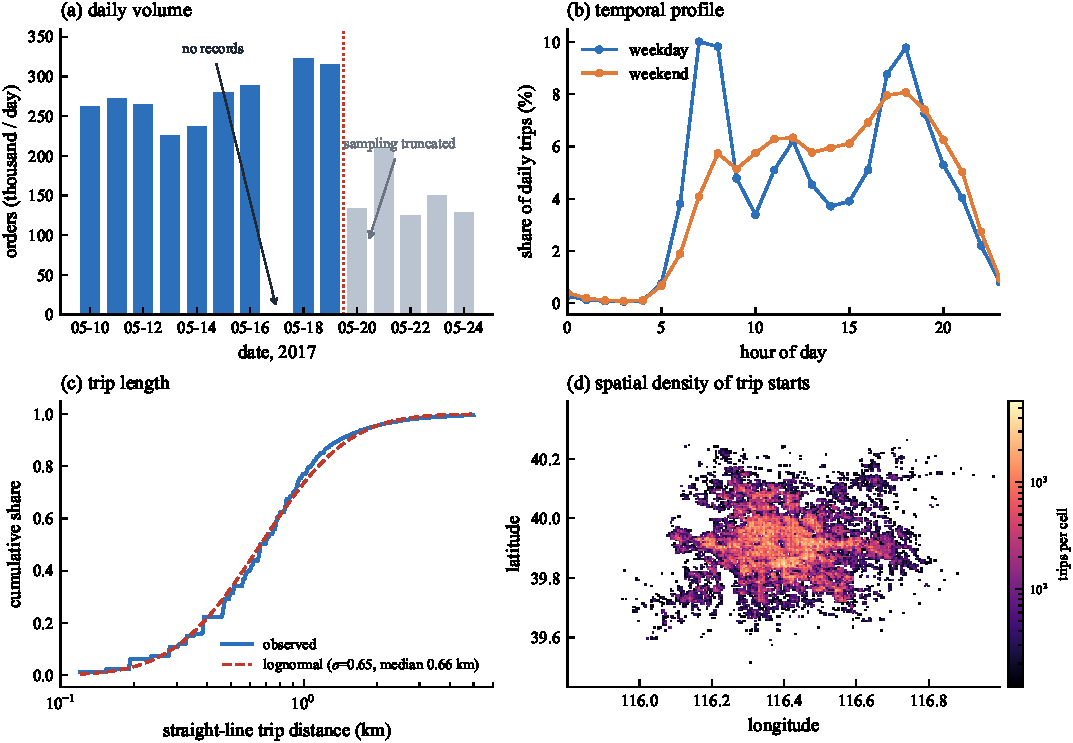
\includegraphics[width=0.9\linewidth]{../figs/fig1_data.pdf}
\caption[The dataset]{The dataset. (a) Daily order volume; 17 May has no records and the sample is
truncated from 20 May. (b) Hourly profile, weekdays against weekends. (c) Empirical
distribution of straight-line trip distance with a fitted lognormal. (d) Spatial
density of trip starts, logarithmic colour scale.}
\label{fig:data}
\end{figure}

\subsection{The sampling rate}

The file is a sample of the operator's orders, not a census. If each order is retained
independently with probability $p$, then every count must be divided by $p$, and the
number of distinct bicycle identifiers understates the fleet. We estimate $p$ from
the bicycles themselves.

For a given bicycle, consider two consecutive orders that both appear in the file.
They are adjacent in the bicycle's true history exactly when no order between them was
dropped, which for independent retention happens with probability $p$. Adjacency is
observable: if the two orders are adjacent, the bicycle was not moved in between, so
the second order must start in the same 153 m geohash cell in which the first ended.
Conversely, a mismatch proves that at least one order is missing. Across all bicycles
with two or more orders, \textbf{12.8\% of consecutive pairs satisfy the
end-equals-next-start test}.

Two biases act in opposite directions and both are small. A bicycle re-parked within
the same 153 m cell after an unobserved trip creates a false match, which makes 12.8\%
an overestimate of the match rate and hence a \emph{lower} bound on $p$; a bicycle
locked a few metres away but across a cell boundary creates a false mismatch. We adopt
$p=0.128$ and treat it as an order-of-magnitude estimate. Section~\ref{sec:sens}
shows that this uncertainty does not propagate into the fleet estimate at all.

\subsection{Fleet size}

The file contains no inventory, so the fleet must be inferred from the pattern of use.
Model each bicycle as being ridden a random number of times per day with mean $\mu$,
Poisson distributed across bicycles and independent across days. A bicycle appears in
the data at least once with probability $1-e^{-\mu}$. With $T$ orders and $D$ distinct
bicycles observed on a day,
\begin{equation}
\frac{T}{D} \;=\; \frac{\mu}{1-e^{-\mu}},
\label{eq:fleet}
\end{equation}
which is strictly increasing in $\mu$ and therefore invertible. For the reference
weekday $T/D=1.478$, giving $\mu=0.840$ and
\begin{equation}
\hat F \;=\; \frac{T}{\mu} \;=\; 343{,}638 \ \text{bicycles}.
\end{equation}

The estimate is invariant to the sampling rate, which is worth showing because it is
the reason the unidentified $p$ does no damage. Under retention probability $p$ the
observed quantities are $T_p=pT$ and $D_p=F(1-e^{-p\mu})$, so
$T_p/D_p=p\mu/(1-e^{-p\mu})$. Inverting \eqnref{eq:fleet} on the observed ratio
returns $p\mu$, and $\hat F=T_p/(p\mu)=T/\mu$. Resampling the orders at rates from 5\%
to 50\% reproduces $\hat F$ within 4\% (Section~\ref{sec:sens}), which confirms the
algebra numerically.

At 343,638 bicycles and $2.14\times10^6$ rides per day, each bicycle is ridden
\textbf{6.2 times per day}. For comparison, a private car is driven three to four times
per day; the fleet is worked hard in the aggregate and idle in the particular, which
is the tension the rest of the paper quantifies.

\subsection{Spatial units}

Two partitions are used, at different resolutions and for different purposes.

\textbf{Cells.} A grid of $0.005^\circ$ (about $555\times426$ m) is laid over the
city. Keeping only cells with at least 50 sampled trips leaves \textbf{5,263 cells},
which contain 95.8\% of the typical-day trips. Cells are the unit at which a rider can
reasonably be asked to change destination (a few hundred metres), so they are used for
the incentive model (Q3) and the parking model (Q4).

\textbf{Zones.} Fifty zones are formed by $k$-means on the cell centroids weighted by
trip volume, and each cell is assigned to its nearest centroid. Zones hold between
604 and 12,119 trips per day and are roughly 4 km across, which is the scale at which a
truck moves bicycles. They are used for rebalancing (Q2).

\tabref{tab:data} collects the descriptive statistics.

\begin{table}[htbp]
\centering
\caption[Data summary after cleaning]{Data summary after cleaning. Distances are straight-line between decoded
endpoints.}
\label{tab:data}
\small
\begin{tabular}{@{}lrl@{}}
\toprule
\textbf{Quantity} & \textbf{Value} & \textbf{Note} \\
\midrule
Order records & 3,213,310 & after bounding-box filter (786 removed) \\
Users & 349,241 & \\
Bicycles & 484,754 & distinct identifiers over 14 days \\
Dates present & 14 & 17 May absent \\
Typical days used & 7 & fully covered weekdays \\
Trips per typical day (sample) & 274,357 & \\
Trips per typical day (scaled) & $2.14\times10^6$ & $p=0.128$ \\
Median trip distance & 0.70 km & lognormal $\sigma=0.65$ \\
90th percentile distance & 1.41 km & \\
Study cells & 5,263 & $\geq50$ trips, $0.005^\circ$ grid \\
Traffic zones & 50 & weighted $k$-means \\
Fleet estimate & 343,638 & Eq.~\eqref{eq:fleet} \\
Rides per bicycle per day & 6.2 & scaled trips / fleet \\
\bottomrule
\end{tabular}
\end{table}

Two remarks on the distance distribution (\figref{fig:data}c). It is close to
lognormal, with an empirical median of 0.70 km and a 90th percentile of 1.41 km, but
the fit is not exact: the lognormal drawn in the figure has $\sigma=0.65$ and a median
of 0.66 km, and the 0.04 km by which it undershoots the empirical median is the
compressed lower tail, because trips shorter than about 150 m cannot be distinguished
from zero at the geohash resolution. This is a measurement floor, not a behavioural
feature, and the gravity model is estimated on the distances that are resolved.

% =============================== 4. Q1 ===============================
\section{Question 1: A Behavioural Model of Riding}\label{sec:q1}

The deliverable of Q1 is a probability law for a trip: when it starts, where it goes,
and how long it lasts. We build it in three layers --- generation, destination,
duration --- and validate the layers jointly against held-out days.

\subsection{Generation: a non-homogeneous Poisson process}

Each cell $i$ emits trips as a Poisson process whose rate $\lambda_{i}(t)$ is constant
on 15-minute intervals. The rate is estimated by the sample mean of the counts in that
interval over the seven typical days,
\begin{equation}
\hat\lambda_{it} \;=\; \frac{1}{7}\sum_{k=1}^{7} N_{it}^{(k)},
\end{equation}
where $N^{(k)}_{it}$ is the number of departures from cell $i$ in interval $t$ on day
$k$. With 5,263 cells and 96 intervals the table has $5.05\times10^{5}$ entries, which
is precisely the level of detail the data support: the average cell-interval contains
0.54 trips, and the profile (\figref{fig:data}b) is bimodal on weekdays, with a sharp
8 a.m. peak, a lunchtime shoulder and an evening peak at 6 p.m., and unimodal on
weekends.

\subsection{Destination: a singly-constrained gravity model}

Conditional on departing from $i$ in time band $h$, a rider chooses destination $j$
with probability
\begin{equation}
P(j\mid i,h) \;=\; \frac{A_j(h)\,e^{-\beta_h d_{ij}}}
                        {\sum_{k} A_k(h)\,e^{-\beta_h d_{ik}}},
\qquad d_{ij}\ \text{in km},
\label{eq:gravity}
\end{equation}
where $A_j(h)$ is the attraction of $j$ in band $h$ and $\beta_h>0$ is the distance
decay. The model is origin-constrained --- the probabilities sum to one over
destinations for every origin --- so the observed origin totals are reproduced exactly
and no balancing procedure is required beyond the denominator.

The exponential form is not an arbitrary choice. If trips are the most probable
allocation of $n_{ih}=\sum_j n_{ijh}$ indistinguishable riders to destinations subject
to a known mean trip length, the maximum-entropy distribution is
\cite{wilson1970}
\begin{equation}
n_{ijh} \;\propto\; A_j(h)\,e^{-\beta_h d_{ij}},
\end{equation}
and $\beta_h$ is the Lagrange multiplier of the distance constraint. It measures how
strongly riders resist distance: a large $\beta_h$ means the destination distribution
is concentrated near the origin.

Attraction is measured, not assumed. We set
\begin{equation}
A_j(h) \;=\; \sum_{n:\,h_n=h} K\!\left(\|c_j-c_{d_n}\|\right),
\end{equation}
a Gaussian kernel ($\sigma=1.2$ cells, about 600 m) over the destinations actually
observed in band $h$, evaluated at the cell centroid $c_j$. The kernel matters because
a destination's pull extends beyond its own cell boundary: a rider heading for a
shopping street will accept any of the cells that front it. Using unsmoothed arrival
counts instead would set $A_j=0$ for 0.3\% of cells in the busiest bands and for 30.6\%
of them at night, forbidding trips that the data plainly contain.

\subsection{Estimation}

Only $\beta_h$ is a free parameter. For a band with trips $\{(i_n,j_n)\}$ it is the
maximiser of the conditional log-likelihood
\begin{equation}
\ell(\beta) \;=\; \sum_{n} \left[\log A_{j_n}(h) - \beta\, d_{i_n j_n}
 - \log \sum_k A_k(h)\,e^{-\beta d_{i_n k}}\right],
\label{eq:mle}
\end{equation}
which is concave in $\beta$; we maximise it by bounded scalar search
\cite{virtanen2020}. The five bands are estimated separately on five randomly chosen
typical days and tested on the remaining two. \tabref{tab:q1} reports the estimates and
the out-of-sample performance.

\begin{table}[htbp]
\centering
\caption[Q1 estimates and held-out performance]{Q1 estimates and out-of-sample performance (two held-out days). Log-loss is
nats per trip; lower is better. ``Attraction only'' is the same model with
$\beta_h=0$.}
\label{tab:q1}
\small
\begin{tabular}{@{}lrrrrrrr@{}}
\toprule
\textbf{Band} & \textbf{Train trips} & $\hat\beta_h$ & \textbf{Gravity} &
\textbf{Distance} & \textbf{Attraction} & \textbf{Uniform} & \textbf{Top-5 hit} \\
 & & (km$^{-1}$) & \textbf{log-loss} & \textbf{only} & \textbf{only} & & \textbf{gravity / dist.} \\
\midrule
00--05 & 18,364 & 2.096 & 3.313 & 3.488 & 7.912 & 8.568 & 0.476 / 0.401 \\
06--09 & 386,102 & 2.014 & 3.512 & 3.646 & 8.083 & 8.568 & 0.399 / 0.339 \\
10--15 & 366,212 & 2.517 & 3.239 & 3.279 & 8.091 & 8.568 & 0.458 / 0.441 \\
16--19 & 428,478 & 2.130 & 3.517 & 3.562 & 8.140 & 8.568 & 0.408 / 0.383 \\
20--23 & 165,671 & 2.364 & 3.360 & 3.395 & 8.185 & 8.568 & 0.455 / 0.438 \\
\bottomrule
\end{tabular}
\end{table}

Three readings of \tabref{tab:q1} matter.

\textbf{Distance is the dominant explanatory variable.} The attraction-only model is
almost useless --- its log-loss is close to the uniform benchmark over 5,263
destinations ($\log 5263=8.57$) --- because in a balanced system the marginal number of
arrivals at a cell says little about where any particular rider is going. Distance
alone already reaches a log-loss of 3.28--3.65.

\textbf{Attraction adds a consistent but modest gain.} Adding $A_j(h)$ improves the
log-loss by 0.035--0.175 nats and the top-five hit rate by 1.7--7.5 percentage points
in every band and on held-out days. The gain is largest in the small hours, when the
destination choice is least constrained by commuting routine, and smallest in the late
evening, when the distance term is already sharp.

\textbf{The decay varies by time of day, and in the expected direction.} Morning has
the weakest decay ($\hat\beta=2.01$): the morning trip is the commute, and commutes are
long. Midday has the strongest ($\hat\beta=2.52$): the midday trip is an errand, and
errands are local. The evening sits between, and late evening recovers some of the
morning's reach as riders return home. This is the behavioural content of the model,
and it is what makes a time-varying formulation necessary: a single $\beta$ would
average the commute and the errand and misdescribe both.

\subsection{Duration}

Ride duration is generated from speed rather than modelled directly. A bicycle travels
the street network, which is about 1.35 times the straight-line distance at the
distances observed here; the speed of a dockless rider is approximately normal with
mean 11.5 km/h and standard deviation 2.5, clipped to $[6,20]$ km/h to remove the
implausible tails. Hence
\begin{equation}
\tau_n \;=\; \frac{1.35\,d_n}{v_n}\times 60 + 1 \quad \text{minutes},
\label{eq:dur}
\end{equation}
with the additive minute standing for locking and unlocking. The resulting
distribution has median 5.9 minutes, 10th percentile 3.0 and 90th percentile 11.9,
which matches the observed distribution of within-day ride durations.

\subsection{Joint validation}

The layers are estimated separately but must be checked together: a model can fit each
margin and still produce impossible trips. We therefore simulate a full typical day
--- draw each trip's time from the Poisson rates, its destination from
\eqnref{eq:gravity}, its duration from \eqnref{eq:dur} --- and compare the simulated
trip-length distribution with the observed one (\figref{fig:q1}a). The two-sample
Kolmogorov--Smirnov statistic is 0.196, and the discrepancy is confined to the
shortest trips, exactly where the geohash floor sits. Given that the model reproduces
the distance distribution, the hourly profile (by construction) and the destination
choice (by the held-out test), it is adequate as the demand engine for Q2--Q4.

\begin{figure}[htbp]
\centering
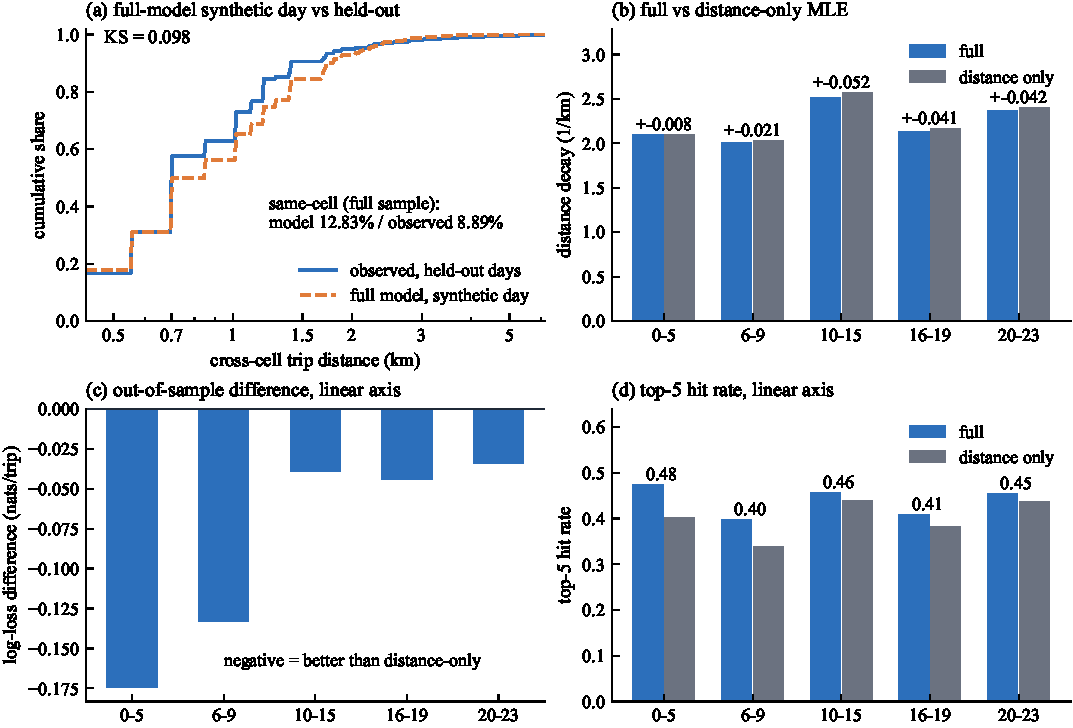
\includegraphics[width=0.9\linewidth]{../figs/fig3_q1_validation.pdf}
\caption[Q1 validation]{Q1 validation. (a) Simulated against observed trip-length distributions.
(b) Estimated distance decay by time band. (c) Out-of-sample log-loss for three
model specifications, logarithmic scale. (d) Top-five destination hit rate.}
\label{fig:q1}
\end{figure}

\subsection{Who is riding}

A single representative rider would misrepresent the system, because the hourly
profile is the superposition of distinct behaviours. We characterise each user by six
features computed over the ten usable days: trips per day, mean trip distance, entropy
of the departure-hour distribution, share of trips in peak hours, share on weekends,
and share of trips that return to the origin cell. $k$-means \cite{lloyd1982} with the
silhouette criterion \cite{rousseeuw1987} selects $k=5$ (silhouette 0.256; the
alternatives $k=3$ and $k=4$ score 0.239 and 0.237), and the resulting classes are
stable across random initialisations.

\begin{table}[htbp]
\centering
\caption[Latent user segments]{Latent user segments (ten days). ``Peak'' is the share of a user's trips
starting in 07--09 or 17--19.}
\label{tab:seg}
\small
\begin{tabular}{@{}lrrrrrr@{}}
\toprule
\textbf{Segment} & \textbf{Users} & \textbf{Share of} & \textbf{Share of} &
\textbf{Trips} & \textbf{Distance} & \textbf{Weekend} \\
 & & \textbf{users} & \textbf{trips} & \textbf{per day} & \textbf{(km)} & \textbf{share} \\
\midrule
Regular multi-purpose & 132,984 & 40.4\% & 51.8\% & 9.18 & 0.84 & 0.19 \\
Heavy short-trip & 49,931 & 15.2\% & 29.6\% & 13.98 & 0.67 & 0.20 \\
Commuter & 67,528 & 20.5\% & 10.6\% & 3.71 & 1.17 & 0.07 \\
Low frequency & 49,396 & 15.0\% & 5.2\% & 2.48 & 0.89 & 0.03 \\
Weekend / leisure & 29,410 & 8.9\% & 2.8\% & 2.25 & 0.92 & 0.79 \\
\bottomrule
\end{tabular}
\end{table}

\figref{fig:seg} and \tabref{tab:seg} show the structure. Two groups generate
four-fifths of all trips. The \emph{regular multi-purpose} user rides 9.2 times a day
--- the profile of a short-distance commuter or a rider who uses the bicycle as a
substitute for walking --- and accounts for 51.8\% of trips. The \emph{heavy
short-trip} user rides 14 times a day over 0.67 km, with a quarter of trips returning
to the same cell: this is the courier-like, errand-heavy behaviour that dominates the
dense core. The \emph{commuter} class rides longer (1.17 km) and concentrates 91\% of
its trips in peak hours but contributes only 10.6\% of volume. The remaining two
classes are peripheral.

This matters operationally rather than descriptively. The peak is made by a minority
of trips --- commuters, 10.6\% of volume --- while the volume is made by riders whose
trips are short and whose destinations are diffuse. An intervention designed to
flatten the peak must target the first group; one designed to reduce total vehicle
movement must target the second. Neither can be inferred from the aggregate profile,
which is why the segmentation is part of the deliverable.

\begin{figure}[htbp]
\centering
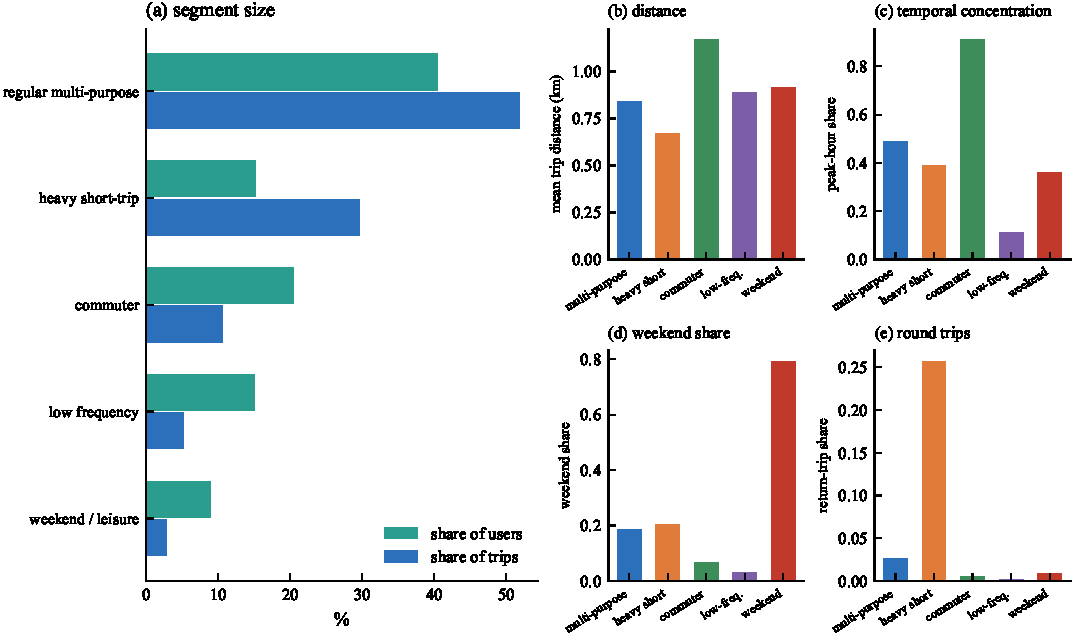
\includegraphics[width=0.9\linewidth]{../figs/fig2_segments.pdf}
\caption[User segments]{User segments. (a) Size of each segment by users and by trips. (b)--(e)
Behavioural signature on four dimensions.}
\label{fig:seg}
\end{figure}

% =============================== 5. Q2 ===============================
\section{Question 2: Optimal Repositioning on a Typical Day}\label{sec:q2}

\begin{figure}[htbp]
\centering
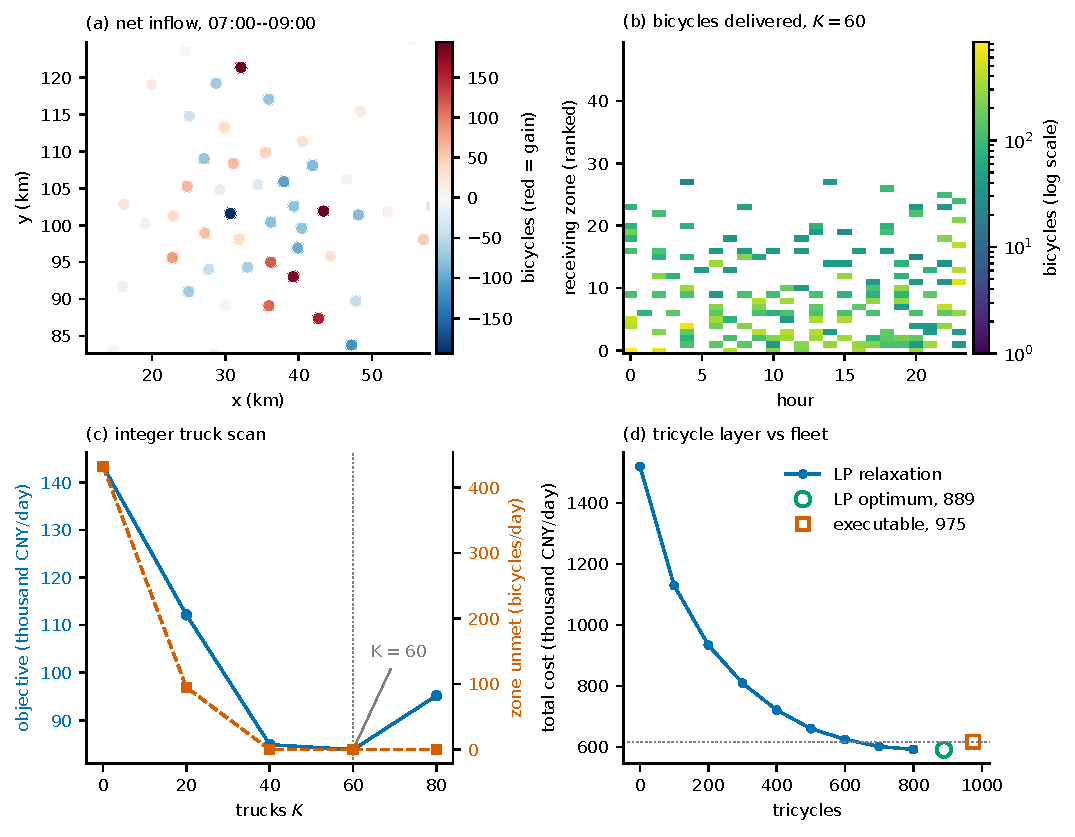
\includegraphics[width=0.9\linewidth]{../figs/fig4_q2.pdf}
\caption[Q2: flow, truck schedule, fleet scans]{Q2. (a) Net flow in the morning peak
by zone: the core gains bicycles, the residential periphery loses them. (b) The
$K=60$ truck schedule: bicycles delivered by hour and receiving zone, from the
integer plan. (c) Integer objective and zone unmet against the truck fleet; $K=60$
is the minimum of the compared grid. (d) Total cost against fleet size from the joint
conserving replay, scaling the executable allocation by 0.70--1.30; the square marks
the 1,233-tricycle executable plan.}
\label{fig:q2}
\end{figure}

\subsection{Two scales of imbalance}

At the
50-zone scale, the flow-only inventory path of each zone,
\begin{equation}
\tilde I_{zt} \;=\; I_{z0} + \sum_{s\le t}\left(a_{zs}-d_{zs}\right),
\label{eq:path}
\end{equation}
never reaches zero from the initial-inventory proxy of 343,638 bicycles; $a$ and
$d$ are the hourly arrivals and departures of a typical day scaled by $1/p$. At that
scale the 50-zone program with no dispatch ($K=0$ in \tabref{tab:q2scan}) leaves
432.23 departures unserved, 0.02\% of 2,132,542.

\textbf{That number is an aggregation artefact.} The same scaled flows and the same
343,638-bicycle inventory, replayed at cell resolution with a conserving process
(departures Poisson,
arrivals generated by served departures, the city total fixed at 343,638 at every
step), leave \textbf{17.40\%} of departures unserved with \emph{no repositioning at
all} (371,129.50 of 2,132,542.19) and \textbf{17.31\%} with the $K=60$ truck plan
running (369,181.08). A zone-level average hides the cell-level shortfall because
cells with opposite imbalances cancel inside a zone. Every statement about service in
this paper is therefore made at cell resolution; the zone model is used only to
\emph{schedule trucks}, which is what it is good for.

\textbf{The truck plan is a balance instrument, not a service instrument.} Running the
$K=60$ plan in the conserving replay removes 1,948 departures (371,129.50 $\to$
369,181.08) for 83,807.74 CNY/day, 43.01 CNY per departure removed against a 6 CNY
service penalty: the trucks pay for end-of-day balance and for nothing else. That is
why the tricycle layer, which can see inside a zone, does the service work.

Rebalancing is therefore not a rescue operation; it is a \emph{reset}, in two layers:
trucks move bicycles between zones, tricycles between cells inside one zone. They are
optimised in that order, because a tricycle cannot undo a zone-level shortage.

\subsection{The truck layer: a time-space network program}

Let $z=1,\dots,50$ index zones and $t=0,\dots,23$ hours. The decision variables are
the inventory $I_{zt}$, the bicycles moved $x_{ijt}$ and the trucks moved $m_{ijt}$ on
arc $(i,j)$ of a sparse zone graph (the eight nearest neighbours of each zone within
9 km; 290 arcs, mean length 5.97 km), the trucks present $n_{zt}$, the unmet
departures $u_{zt}$, and the end-of-day deviations $dp_z,dm_z$.

{\allowdisplaybreaks
\begin{align}
\min\quad
& c_{\text{km}}\sum_{t}\sum_{(i,j)} d_{ij}\,m_{ijt}
+ c_{\text{load}}\sum_t\sum_{(i,j)} x_{ijt}
+ w\sum_t\sum_z u_{zt}
+ c_{\text{dev}}\sum_z\left(dp_z+dm_z\right)
+ f K \label{eq:q2obj}\\
\text{s.t.}\quad
& I_{z,0} = I_{z0}, \label{eq:q2init}\\
& I_{z,t+1} = I_{z,t} + a_{zt} - \left(d_{zt}-u_{zt}\right)
  - \sum_{j} x_{zjt} + \sum_{i} x_{izt}, \label{eq:q2bal}\\
& \sum_j x_{zjt} + d_{zt} - u_{zt} \;\le\; I_{z,t}, \label{eq:q2serv}\\
& x_{ijt} \;\le\; Q\,m_{ijt}, \label{eq:q2cap}\\
& \sum_{j} m_{zjt} \;\le\; n_{zt}, \label{eq:q2truck}\\
& n_{z,t+1} = n_{zt} - \sum_j m_{zjt} + \sum_i m_{izt},
  \qquad \sum_z n_{z,0} = \sum_z n_{z,23} = K, \label{eq:q2fleet}\\
& \big[I_{z,23} + a_{z,23} - (d_{z,23}-u_{z,23})
   - \textstyle\sum_j x_{zj,23} + \sum_i x_{iz,23}\big] - I_{z0} = dp_z - dm_z,
  \label{eq:q2dev}\\
& I,u,dp,dm \ge 0,\qquad x,m,n \in \mathbb{Z}_{\ge 0}. \notag
\end{align}}

The objective prices five things. $c_{\text{km}}=6$ CNY per truck-kilometre is the
running cost; $c_{\text{load}}=0.5$ CNY per bicycle loaded and unloaded is handling;
$w=6$ CNY per unmet departure is a service penalty set above the cost of moving a
bicycle; $c_{\text{dev}}=3$ CNY per bicycle of end-of-day drift, linearised by $dp,dm$,
penalises leaving the system out of balance; and $f=600$ CNY per truck per day is the
ownership cost of a truck, charged on $K$.

The constraints are the physics. \eqnref{eq:q2bal} is conservation of bicycles;
\eqnref{eq:q2serv} is the event-order constraint: a truck may take away only bicycles
present at the start of the hour, before that hour's departures are served;
\eqnref{eq:q2cap} couples bikes to trucks ($Q=40$ bicycles per truck);
\eqnref{eq:q2truck}--\eqnref{eq:q2fleet} conserve the truck count, with $K$ at the
start and at the end of the day but no per-zone requirement; end-of-day positions are
matched to the start-of-day ones by the deadhead relocation reported below, outside the
objective; \eqnref{eq:q2dev} defines the end-of-day deviation that
makes the plan a reset. Bicycles, trucks and truck presence are integer variables; as
a continuous program it would be cheaper but would describe fractions of a
truck and of a bicycle.

The continuous LP plan, re-checked
on its own demand, violates the stock constraint in 3 of 1,200 zone-hours and would
take 717.54 bicycles out of zones that do not have them. The integer plan has zero
violations of every constraint: maximum load 40 bicycles, maximum trip 46.92 minutes
against the 60-minute hour, truck-conservation residual 0, at least 0.81 bicycles of
event-order slack in every zone-hour, and minimum inventory 1,891.36. The LP relaxation
at $K=60$ costs 82,968.0671 and the MILP 83,807.7438, a gap of 839.68 CNY (1.01\%). The plan also has an end-of-day deadhead of 1,023.76 truck-kilometres
(6,142.58 CNY), which is not in the objective and is reported separately; repeating the
daily plan requires it. The truck cost is common to both totals in the comparison, and
the deadhead enters neither: adding it to both sides would leave the absolute saving
unchanged but lower the percentage below the 65.38\% quoted.

\subsection{Trucks alone: the single-layer baseline}

\tabref{tab:q2scan} scans the integer fleet on the five grid points that were solved.
$K=0$ is the no-dispatch point; $K=60$ is the minimum of the compared grid and the
baseline against which the tricycle layer is evaluated, not the Q2 recommendation
once tricycles are available.

\begin{table}[htbp]
\centering
\footnotesize
\caption[Integer truck scan]{Integer truck plan by fleet size. ``Zone unmet'' is
the unmet departures of the 50-zone model, priced at 6 CNY; the objective includes the
fixed cost $600K$, the kilometre and loading costs, and the deviation. The LP relaxation
at $K=60$ costs 82,968.0671.}
\label{tab:q2scan}
\scriptsize
\begin{tabular}{@{}rrrrrr@{}}
\toprule
$K$ & \textbf{Moved} & \textbf{Truck-km} & \textbf{Zone unmet} & \textbf{Dev} &
\textbf{Objective} \\
\midrule
0  & 0      & 0.00     & 432.23 & 46,930.39 & 143,384.53 \\
20 & 9,503  & 1,767.02 & 95.01  & 28,083.10 & 112,172.98 \\
40 & 19,104 & 4,097.39 & 0      & 8,907.88  & 84,860.02 \\
\textbf{60} & \textbf{24,949} & \textbf{5,659.17} & \textbf{0} &
\textbf{459.41} & \textbf{83,807.74} \\
80 & 24,863 & 5,495.85 & 0      & 586.96    & 95,167.44 \\
\bottomrule
\end{tabular}
\end{table}

At $K=60$ the 24,949 relocated bicycles cost
5,659.17 truck-kilometres, and the end-of-day deviation falls from 46,930.39 at $K=0$
to 459.41: the objective is dominated by balance, not by service, because the zone
model has almost no unmet demand to remove. More trucks bring diminishing returns
after 60: $K=80$ adds 11,359.70 CNY and moves 86 fewer bicycles.

The hold-out replay fixes the plan on the five training days and replays it on the
two held-out days. On 12 May, at
0.9291 times the design volume, it leaves 704.74 departures unserved and ends
53,255.64 bicycles away from balance; on 19 May, at 1.1066 times the design volume, it
leaves 14,232.37 unserved, 0.60\% of that day's departures, and 51,718.20 away from
balance. No zone-hour hits the truck capacity in either replay. The service cost of a
volume surprise is small in percentage terms, but the end-of-day balance deteriorates
sharply: the plan is built for the typical day, not for the tail.

\subsection{The tricycle layer: replacing within-zone walking with a fleet}

The truck plan equalises zone totals. Inside a zone, riders can already borrow a
bicycle up to 300 m away, but the 300 m radius reaches no neighbour cell centre on this
grid, so walking cannot move a bicycle across a cell boundary. The tricycle layer is
therefore a within-zone transport problem. A tricycle carries $Q_{\text{tri}}=20$
bicycles, travels at 15 km/h, needs 0.5 minutes per bicycle handled, makes trips of at
most 5 km, and operates from 07:00 to 20:00. Its cost is 300 CNY per tricycle-day,
0.2 CNY per vehicle-kilometre ($c_{\text{km}}$), and the same 6 CNY penalty
($w_{\text{tri}}$) on any cell-level departure left unserved. The layer is solved zone
by zone; the truck layer is held fixed at the $K=60$ plan.

A deficit cell $a$ is paired with the 12 nearest
stock-holding cells $b$ inside the trip limit; $y_{ab}$ bicycles move from $b$ to $a$,
$u_a$ departures stay unserved, $e_a$ the departure still unmet after trucks and
walking, $I_b$ the donor stock at the hour start, $d_{ab}$ the distance,
$\nu_z$ the zone's tricycles, and $\theta_{ab}$ the tricycle-hours one bicycle on
arc $ab$ occupies: loaded leg out, empty return, one full load, plus handling at both
ends. For each zone-hour,
\begin{equation}
\begin{aligned}
&\min\;\sum_{ab}\frac{c_{\text{km}}}{Q_{\text{tri}}}\,d_{ab}\,y_{ab}
  +w_{\text{tri}}\sum_a u_a\\
&\text{s.t.}\;\;\sum_b y_{ab}+u_a=e_a,\qquad
\sum_a y_{ab}\le I_b,\qquad
\sum_{ab}\theta_{ab}\,y_{ab}\le\nu_z ,
\end{aligned}
\label{eq:q2tri}
\end{equation}
with flows and unmet non-negative. The LP solution is rounded to whole bicycles under
each donor's integer stock and split into trips of at most $Q_{\text{tri}}$. The fixed
list is assigned to the zone's tricycles by earliest finish inside the shift, and the
smallest integer fleet that places every trip replaces the fractional count zone by zone.

The joint conserving replay is optimised by coordinate descent over integer per-zone
fleets: each candidate changes one zone by $\pm1$ or $\pm2$ tricycles and is evaluated
by a full 24-hour simulation of the city, because a fleet change alters the served
departures and therefore every later arrival. From the scaled start (1,271 tricycles,
1.10 times the earlier allocation) the descent settles
at \textbf{1,196 tricycles}, a layer of 707,118.68 and a total of 790,926.43, with
57,759.37 cell-level departures unserved and 8,812.18 tricycle-kilometres. That
allocation is not yet executable: the per-zone trip schedule cannot always be run at the
fleet the descent evaluates, so each zone is raised to the smallest integer fleet at which
its schedule places every trip. The executable plan is \textbf{1,233 tricycles}, a layer
of \textbf{712,063.25} --- 369,900 fixed, 1,772.82 kilometre cost and 340,390.43 the 6 CNY
penalty on 56,731.74 unserved --- and a total of \textbf{795,870.99 CNY/day}, a saving of
\textbf{1,503,023.20 (65.38\%)} against the 2,298,894.20 no-tricycle baseline. The
executable fixed point costs 4,944.57 (0.62\%) more than the descent allocation and
serves 1,027.64 more departures; it is the plan we report.

The gap between the two allocations is the price of executability, and it is small. The
37 added tricycles cost 11,100 in fixed cost and 10.38 in kilometres, while the
1,027.64 departures they serve are worth 6,165.82 in penalty; the net is the
4,944.57 difference. The conserving replay values a tricycle more highly than the zone
model did, because it sees the cell-level shortfall that the zone totals cancel; the
6 CNY penalty is doing the work.

\subsection{The three schemes on their own calibers}

\tabref{tab:q2schemes} puts the schemes side by side. The two panels are
\emph{different accounting calibers}: the truck plan was optimised in the zone model,
where it removes all 432.23 unmet departures at $K=0$ and costs 83,807.74 at $K=60$;
the same plan, priced in the cell model, carries a cell deficit of 369,181.08 that the
zone model cannot see, and the two-tier plan is the only row that removes most of it.

\begin{table}[htbp]
\centering
\footnotesize
\caption[Q2 schemes]{Q2 schemes at two calibers. Panel A is the 50-zone model in which
the truck plan is optimised; Panel B is the cell-level conserving model, with the same
$K=60$ truck plan and the cell deficit priced at 6 CNY. ``Truck'' is the zone-level
truck objective, including its own zone penalty and deviation in Panel A; ``tricycle
operating'' is fixed, kilometre and handling cost; ``cell penalty'' is 6 CNY times the
cell-level unmet. The 2,298,894.20 baseline is the cell-level cost of the truck-only
plan, not the 83,807.74 zone-level objective.}
\label{tab:q2schemes}
\scriptsize
\begin{tabular}{@{}lrrrrr@{}}
\toprule
\textbf{Scheme} & \textbf{Fleet} & \textbf{Truck} & \textbf{Tricycle operating} &
\textbf{Cell penalty} & \textbf{Total} \\
\midrule
\multicolumn{6}{@{}l}{\emph{Panel A: zone-level caliber (unmet 432.23 at $K=0$, 0 at $K=60$)}}\\
No dispatch & $K=0$ & 143,384.53 & --- & --- & 143,384.53 \\
Trucks only & $K=60$ & 83,807.74 & --- & --- & 83,807.74 \\
\midrule
\multicolumn{6}{@{}l}{\emph{Panel B: cell-level caliber (cell unmet shown in the last column)}}\\
Trucks only & $K=60$ & 83,807.74 & --- & 2,215,086.45 & 2,298,894.20 \\
Two-tier & $K=60$, 1,233 tricycles & 83,807.74 & 371,672.82 & 340,390.43 &
\textbf{795,870.99} \\
\bottomrule
\end{tabular}

\smallskip
\raggedright Cell-level unmet: 369,181.08 for trucks only; \textbf{56,731.74} for the
two-tier plan.
\end{table}

Panel A gives the single-layer result: 143,384.53 at $K=0$ against 83,807.74 at $K=60$,
a saving of 59,576.79 (41.55\%). Panel B gives the two-tier result: 2,298,894.20
against 795,870.99, a saving of 1,503,023.20 (65.38\%). The two savings answer different
questions: 41.55\% is what trucks do for the zone model, 65.38\% what the tricycle
layer adds once the zone model's blind spot is priced, and neither is a system-level
claim.

\subsection{Uncertainty and the limits of the number}

The numbers above are a planning midpoint, not an expectation or a median. The joint
sample of Section~\ref{sec:sens} re-evaluates the executable allocation inside the
conserving replay at every draw, with the fleet held at its 1,233 tricycles, so the
interval describes the cost of the reported plan under parameter uncertainty, not the
cost of a re-optimised fleet. Across the 128 joint draws the two-tier total has
P5/P50/P95 \textbf{316,247 / 585,792 / 1,242,903} CNY/day, the executable unmet
1,178 / 14,322 / 111,974, and the saving share $-0.5757$ / 0.2458 / 0.7352. The 65.38\%
is therefore a midpoint: in 36 of the 128 draws the two-tier plan costs more than no
tricycles at all --- draws in which the fleet would be cut, not kept. The anchors are
small: the reference draw's truck objective is the LP's 82,968.07 rather than the integer
plan's 83,807.74, a shift of 839.67 on every draw, and the replay conserves the city
total to within 0.0004 of 343,638 in every draw.

Two boundaries follow. The 1,233-tricycle fleet is the smallest executable fixed point
of the descent allocation, not a global optimum: the coordinate descent is a local
search over integer fleets, and the joint curve of Figure~\ref{fig:q2}(d) is flat
around the optimum. And the intervals are fixed-fleet intervals --- every draw pays for
1,233 tricycles and the truck plan is re-solved on the draw's demand --- so a draw that
re-optimised the fleet would lie below them; they are an outer bound on the
uncertainty of the reported plan.

% =============================== 6. Q3 ===============================
\section{Question 3: Paying Riders to Move Bicycles}\label{sec:q3}

\subsection{What an incentive can and cannot do}

A truck can carry a bicycle ten kilometres. A rider can be persuaded to end a trip a
few hundred metres from where she intended, and no more: the reward would have to be
absurd to make someone ride across the city. The two instruments therefore operate at
different scales, and the right way to combine them is to ask how much of the
rebalancing problem each can absorb.

This fixes the unit of analysis. The deficit must be measured at the cell, in the hour
in which the cell loses bicycles, and the pool of candidate riders must be measured in
the same cell and the same hour. Measuring either over the whole day, as one is tempted
to do, inflates the pool by an order of magnitude and makes the incentive look free.

\subsection{The deficit to be absorbed}

For each cell $c$ let $n_{ct}=a_{ct}-d_{ct}$ be the net hourly flow and
\begin{equation}
\Delta_c \;=\; \max_t\left(0,\,-n_{ct}\right),
\qquad
N \;=\; \sum_c \Delta_c \;=\; 216{,}344 .
\label{eq:deficit}
\end{equation}
$\Delta_c$ is the number of bicycle-positions cell $c$ must receive during its own worst
hour to avoid drawing down its stock, and $N$ is the daily workload of a perfect
incentive scheme that ignored inventory. Of the 5{,}263 cells, 5{,}192 have $\Delta_c>0$;
the distribution is skewed, with median 17.9, 90th percentile 98.2 and 99th percentile
323.3 bicycles per hour.

\subsection{Will a rider accept?}

A rider whose trip is about to end at cell $j$ is offered $r$ CNY to end instead at
deficit cell $c$ at distance $d_{jc}$. The detour costs her the extra riding time plus
the extra walk,
\begin{equation}
\tau(d) \;=\; \frac{d}{v}\,\times 60 \;+\; \frac{1000\,d}{w}
\quad\text{minutes},\qquad v=10\ \text{km/h},\ w=80\ \text{m/min},
\label{eq:tau}
\end{equation}
and she accepts with the logit probability
\begin{equation}
\pi(d,r) \;=\; \frac{1}{1+\exp\left[-\left(\kappa r-\rho\,\tau(d)-c_0\right)\right]},
\qquad \kappa=2.0,\ \rho=0.35,\ c_0=0.8 .
\label{eq:logit}
\end{equation}
The parameters say that a rider values one yuan at two units of utility, one minute of
detour at 0.35 units, and carries 0.8 units of inertia against changing her plan. They
are not identified from our data --- no reward was offered in May 2017 --- and are
swept in Section~\ref{sec:sens}; what matters is the shape, not the level.

At the optimal reward derived below ($r=1.20$ CNY) acceptance falls from 78\% for a
50 m detour, through 54\% at 225 m, to 21\% at 450 m. The gradient is the whole story:
the scheme recruits the riders who were nearly going there anyway, and pays more and
more for the marginal ones.

\subsection{The supply curve of voluntary relocations}

Trips end at every distance in $[0,R]$, and the ones that end closest accept most
readily. We therefore discretise the catchment into six detour bands
$[0,50),[50,100),\dots,[300,450)$ m, count the trips $n_{cb}$ ending in band $b$
around cell $c$ during $c$'s deficit hour, and obtain the expected placements at
reward $r$ as
\begin{equation}
q(r) \;=\; \sum_c \min\left\{\Delta_c,\ \sum_b n_{cb}\,\pi(\bar d_b,r)\right\},
\label{eq:supply}
\end{equation}
where $\bar d_b$ is the band midpoint. The minimum enforces that a cell cannot absorb
more bicycles than it needs; the inner sum is the number of riders who would accept.
The function $q(r)$ is increasing and concave, and it saturates: no reward, however
large, can move a rider who is not there.

\begin{table}[htbp]
\centering
\caption[The supply curve at 450 m]{The supply curve at 450 m. ``Bill'' is $r\,q(r)$; the last column is the
marginal cost $\Delta(rq)/\Delta q$ over the interval since the previous row, to be
compared with the truck's 3.48 CNY.}
\label{tab:supply}
\small
\begin{tabular}{@{}rrrrr@{}}
\toprule
\textbf{Reward $r$ (CNY)} & \textbf{Placements $q$} & \textbf{Share of $N$} &
\textbf{Bill (CNY)} & \textbf{Marginal cost} \\
\midrule
0.2 & 51{,}380  & 23.7\% & 10{,}276  & --- \\
0.4 & 64{,}938  & 30.0\% & 25{,}975  & 1.16 \\
0.6 & 78{,}709  & 36.4\% & 47{,}226  & 1.54 \\
0.8 & 92{,}036  & 42.5\% & 73{,}629  & 1.98 \\
1.0 & 104{,}409 & 48.3\% & 104{,}409 & 2.49 \\
1.5 & 128{,}873 & 59.6\% & 193{,}310 & 3.63 \\
2.0 & 143{,}615 & 66.4\% & 287{,}229 & 6.37 \\
3.0 & 153{,}654 & 71.0\% & 460{,}961 & 17.31 \\
3.5 & 154{,}846 & 71.6\% & 541{,}961 & 67.95 \\
\bottomrule
\end{tabular}
\end{table}

\tabref{tab:supply} gives the curve. Two properties drive the recommendation.

\textbf{The first half is cheap.} The first 100{,}000 relocations cost 104{,}409 CNY,
an average of 1.0 CNY each, and at that scale the marginal placement still costs 2.5
CNY --- below the truck's 3.48, because there are enough riders passing within 100 m of
the deficit cells.

\textbf{The second half is not.} Beyond about 100{,}000 placements the cheap riders are
exhausted, and because the reward is uniform the platform must raise it for everyone in
order to recruit the few who are far away. The marginal cost of an extra placement then
rises faster than the reward itself: 3.63 CNY at $r=1.5$, 6.37 at $r=2.0$, 17.31 at
$r=3.0$. The curve ends in a wall at 71.6\%, where the pool of qualifying trips is
exhausted.

\subsection{The optimal mix}

The platform chooses $r$ to minimise the incentive bill plus the cost of moving the
residual by truck:
\begin{equation}
\min_{r\ge0}\ \ r\,q(r) \;+\; c_{\text{truck}}\left(N-q(r)\right),
\qquad c_{\text{truck}}=3.48\ \text{CNY}.
\label{eq:mix}
\end{equation}
The first-order condition is that the marginal cost of an incentive placement equals
the truck cost; on \tabref{tab:supply} that happens between $r=1.0$ and $r=1.5$. Solving
numerically gives
\begin{equation}
\boxed{\ r^*=1.20\ \text{CNY},\qquad q^*=115{,}385\ \text{placements}\ (53.3\%),\qquad
\text{bill}=138{,}462\ \text{CNY}\ }
\end{equation}
with a marginal cost of 3.46 CNY, within 1\% of the truck. The remaining 100{,}959
bicycles must be moved by truck for 351{,}116 CNY, so the daily cost is \textbf{489{,}578
CNY against 752{,}404 for an all-truck policy --- a saving of 34.9\%}
(\figref{fig:q3}c).

The optimum is not a corner solution, which is the useful part. Incentives do not
replace trucks; they remove the cheapest half of the trucks' work, and the two
instruments meet where their marginal costs are equal, as they should.

\subsection{Why the ceiling is physical}

At $r=3.5$ the scheme buys 71.6\% of the deficit and then stops. The remaining 28\%
is not a pricing failure: those cells have too few trips ending nearby in their deficit
hour for any reward to reach them. Widening the catchment helps only slowly
(\figref{fig:q3}d): 450 m covers 71.9\%, 600 m covers 83.3\%, 850 m covers 92.2\%, and
95\% requires a 1{,}025 m detour --- a walk of thirteen minutes, which no plausible
reward makes acceptable.

This is the correct division of labour between the instruments. Incentives should be
targeted at cells whose deficit is small relative to the traffic passing through them
--- the dense core, where a few hundred metres of redirection recruits thousands of
riders. Sparse peripheral cells, where the deficit is large and the passing traffic
thin, belong to the trucks.

\subsection{The scheme}

The mechanism that follows from the analysis has five elements.

\begin{enumerate}[leftmargin=1.6em]
\item \textbf{A uniform reward of 1.2 CNY}, paid on completion, credited to the
  account, and about the price of a ride. Uniformity matters: a personalised reward
  would extract more surplus but is perceived as unfair and invites gaming.
\item \textbf{A target set, not a target point.} The reward is offered for ending
  inside any cell in the current deficit list, recomputed hourly from the demand model
  of Section~\ref{sec:q1}. The list is exactly the set of cells with $\Delta_c$ above a
  threshold, which is what focuses the money where it is needed.
\item \textbf{A verified end.} The reward is paid only if the trip ends inside the
  electronic fence (Section~\ref{sec:q4}) of a target cell and the origin is outside
  it, which rules out the trivial strategy of riding in a circle.
\item \textbf{A daily cap} of three rewarded trips per user, which prevents a small
  number of users from absorbing the budget and keeps the scheme a broad-based nudge.
\item \textbf{A hard budget} of 140{,}000 CNY per day, which at $r=1.2$ is exactly the
  volume the analysis recommends; any surplus is carried to the next day.
\end{enumerate}

\begin{figure}[htbp]
\centering
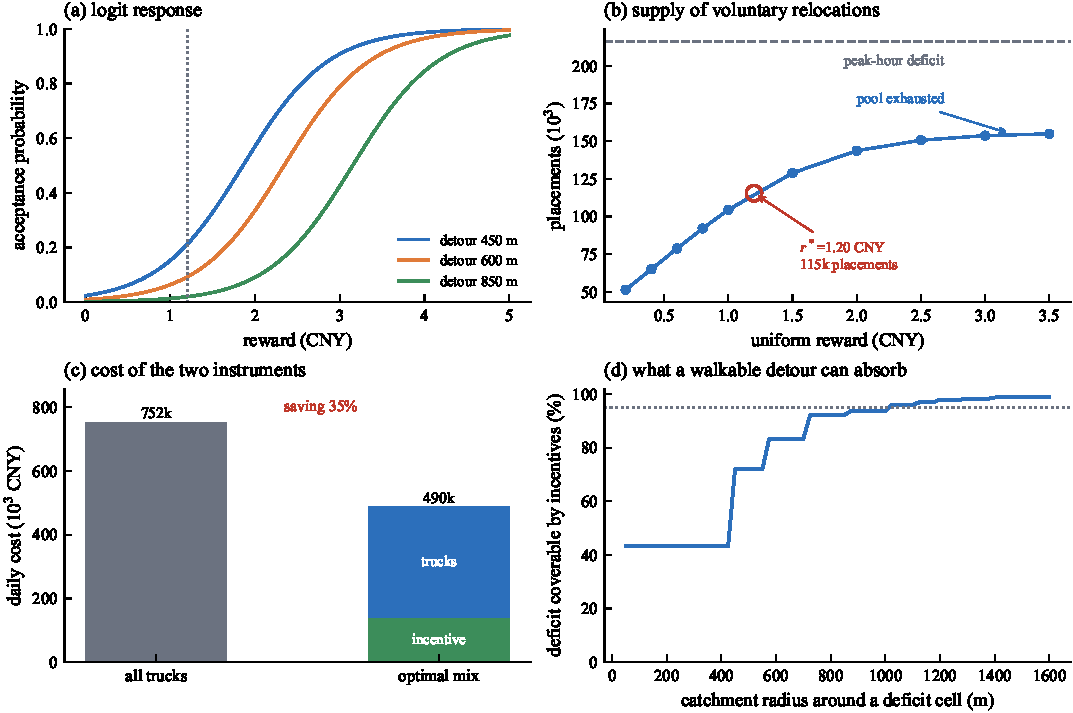
\includegraphics[width=0.9\linewidth]{../figs/fig5_q3.pdf}
\caption[Q3: acceptance, reward and savings]{Q3. (a) Acceptance probability against reward, for three detour distances.
(b) The supply curve of voluntary relocations; the dashed line is the peak-hour
deficit and the circle is the optimum. (c) Daily cost of an all-truck policy and of the
optimal mix. (d) Share of the deficit reachable within a catchment radius.}
\label{fig:q3}
\end{figure}

% =============================== 7. Q4 ===============================
\section{Question 4: Siting and Sizing Electronic Fences}\label{sec:q4}

\subsection{Parking demand is the arrival process}

A dockless bicycle occupies space where its trip ends, and it stays there until someone
rides it away. The demand for parking at a cell is therefore the arrival process ---
which the model of Section~\ref{sec:q1} predicts --- and the capacity of a fence is
the number of bicycles that can be standing inside it at the worst moment of the day.

Capacity is sized by Monte Carlo. For a candidate fence serving a set $S$ of cells we
draw Poisson arrivals and departures on the 15-minute grid,
\begin{equation}
o_{t+1} \;=\; \max\left\{0,\ o_t + A_t - D_t\right\},
\qquad A_t\sim\text{Poisson}\!\left(\textstyle\sum_{c\in S}a_{ct}\right),
\quad D_t\sim\text{Poisson}\!\left(\textstyle\sum_{c\in S}d_{ct}\right),
\end{equation}
record the peak $\max_t o_t$ over 96 intervals, repeat 300 times, and set the capacity
to the 95th percentile of the simulated peaks. Two conventions are worth stating. The
occupancy starts at zero, which is consistent with the nightly reset of
Section~\ref{sec:q2}: fences are emptied overnight and refilled by the day's arrivals.
And the arrival rate is the scaled one, $1/p$ times the sample, so the capacities are
those of the real system rather than of the sample.

\subsection{Where to put the fences}

Siting is a maximal-coverage problem. A fence at cell $c$ with walking radius $R$
serves every arrival whose destination lies within $R$ of $c$; the planner chooses a
set of fences to cover as many arrivals as possible. The problem is NP-hard but its
objective is submodular, so the greedy algorithm --- repeatedly place the fence that
covers the most still-uncovered arrivals --- attains at least $(1-1/e)=63.2\%$ of the
optimum \cite{nemhauser1978}. With 5{,}263 cells and 2{,}500 candidate sites the greedy
pass runs in seconds and the bound is comfortable.

\begin{table}[htbp]
\centering
\caption[Fence plans]{Fence plans. Coverage is the share of daily arrivals inside some fence's
walking radius; capacity is the Monte-Carlo 95th-percentile peak occupancy.}
\label{tab:fence}
\small
\begin{tabular}{@{}rrrrrr@{}}
\toprule
\textbf{Radius $R$} & \textbf{Fences} & \textbf{Coverage} &
\textbf{Total slots} & \textbf{Median slots} & \textbf{Max slots} \\
\midrule
250 m & 505 & 39.0\% & 249{,}860 & 397 & 3{,}261 \\
450 m & 626 & 75.3\% & 344{,}463 & 417 & 4{,}827 \\
650 m & 537 & 83.0\% & 342{,}606 & 489 & 6{,}038 \\
\bottomrule
\end{tabular}
\end{table}

\tabref{tab:fence} and \figref{fig:q4} give the result. A walking radius of 450 m ---
about six minutes, the usual catchment of a transit stop --- covers three-quarters of
arrivals with 626 fences. Tightening to 250 m covers only 39\% even with 505 fences,
because the demand is concentrated in a few hundred cells and a small radius cannot
bridge between them; widening to 650 m covers 83\% with 537 fences, but at a walking
distance riders will not accept for a 700 m trip.

The coverage curves in \figref{fig:q4}b show sharply diminishing returns after about
400 fences. The first 200 fences, placed on the densest cells, cover 39.1\% of
arrivals; the next 200 add 21 percentage points; the last 200 add 14. There is no
layout that covers everything: a quarter of all arrivals end in cells more than 450 m
from every chosen fence, and those cells need either no fence or a shared rack.

\begin{figure}[htbp]
\centering
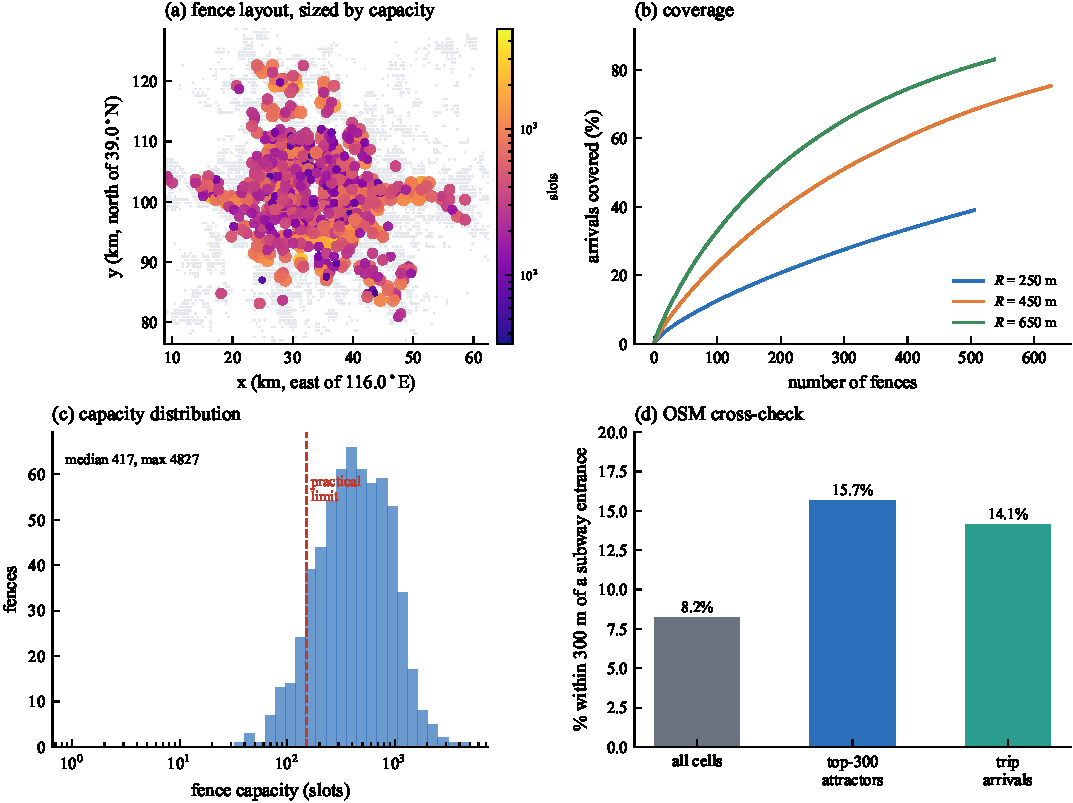
\includegraphics[width=0.9\linewidth]{../figs/fig6_q4.pdf}
\caption[Q4: the 626-fence layout and capacity]{Q4. (a) The 626-fence layout at $R=450$ m, markers sized and coloured by
capacity. (b) Coverage against the number of fences for three walking radii. (c)
Distribution of fence capacity; the dashed line is the 150-slot practical limit. (d)
External check: share of cells, of the top-300 attractors, and of arrivals within
300 m of a subway entrance.}
\label{fig:q4}
\end{figure}


\subsection{How large must each fence be}

The capacities in \figref{fig:q4}c are the most uncomfortable result in this paper.
The median fence needs \textbf{417 slots} and the largest needs \textbf{4{,}827}. At
1.4 m$^2$ per bicycle --- the footprint of a parked bicycle plus its access aisle ---
the plan requires 48.2 hectares of land, the equivalent of 67 football pitches, and the
largest single fence would occupy 0.7 hectares.

The total is not the problem; the distribution is. Every bicycle in the fleet must
stand somewhere, so a 95th-percentile peak, summed over the city, cannot be far from
the fleet: 344{,}463 slots against 343{,}638 bicycles is a 0.2\% margin, and the
agreement is a check on the sizing rather than a coincidence. The
same accounting makes the totals in \tabref{tab:fence} uninformative about layout: the
650 m plan needs 342{,}606 slots and the 450 m plan 344{,}463, within 0.6\% of each
other, because both serve nearly the whole fleet; only the 250 m plan is smaller, and
only because it leaves 61\% of arrivals outside any fence. But
a plan that concentrates 5{,}000 slots on one plaza has not solved parking; it has
formalised the bicycle mountain that electronic fencing was meant to prevent. The
capacity distribution is heavy-tailed because arrivals are: the busiest 10\% of cells
receive 40\% of all trips.

We therefore recommend a \emph{capped} layout rather than an uncapped one. A street
corner can plausibly hold 150 slots --- about 210 m$^2$, a plot ten by twenty-one
metres, the largest a rider can cross in a minute --- and on the uncapped plan
\textbf{89.8\% of fences would exceed it}. Capping instead diverts the excess to the
next fence, and the diversion is exactly the incentive mechanism of
Section~\ref{sec:q3} with the sign reversed: the same reward that fills a deficit cell
can empty an overfull fence, paying the rider to end where there is space.

\subsection{External validation with OpenStreetMap}

The layout is only as good as the demand surface it is built on, and the demand surface
comes from a single operator's data. An independent check is available: if the model's
attractors are real places, they should sit near public transport.

We queried the OpenStreetMap Overpass API for all nodes tagged
\texttt{railway=subway\_entrance} in the study bounding box on 11 November 2026 and
obtained \textbf{1{,}097 entrances} \cite{osm}. The comparison (\figref{fig:q4}d) is
striking. Only 8.2\% of cells lie within 300 m of an entrance, but 15.7\% of the 300
busiest destination cells do --- nearly twice the base rate --- and the median distance
from a top-100 attractor to a subway entrance is \textbf{0.50 km}, against 1.21 km for
a cell chosen at random. Fourteen percent of all arrivals end within 300 m of an
entrance.

The model therefore locates demand where the city's transport infrastructure says it
should be. This does not validate the magnitudes --- an external source cannot do that
--- but it validates the geography, which is what the fence layout depends on.


% =============================== 8. Q5 ===============================
\section{Question 5: What Competition Does to the Problem}\label{sec:q5}

\subsection{Three things competition can break}

The five questions were answered for a single operator holding the whole market.
Competition can affect availability, parking capacity and information, and the three are
not the same kind of claim: availability is a stochastic statement about stockouts,
parking capacity a deterministic one about slots, information a statement about what
any firm can estimate. We simulate the second at the Q4 plan's own resolution and treat
the first and third as arguments whose direction we can state, not whose magnitude we
can measure.

\subsection{A cell-resolution mismatch experiment}

The Q4 plan is fixed: 3,500 sites, 150 slots each, $R=450$ m, initial-inventory proxy
343,638. Two platforms share the market equally (share $s=0.5$), each drawing Poisson
arrivals and departures at half rate and holding half of every cell's inventory. Three
institutions are compared:
\begin{itemize}[leftmargin=1.2em,itemsep=0pt]
\item \textbf{independent} --- each platform owns a 150-slot fence at each open site and
  only its own bicycles park there;
\item \textbf{independent\_equal} --- the same, but 75 slots per platform, so the concrete
  per site equals the shared regime's 150 and the comparison isolates pooling, not total
  capacity;
\item \textbf{shared} --- one 150-slot fence per site, both platforms park in it, riders
  still take only their own bicycles, and overflow is rationed in proportion to that
  step's arrivals. Sharing pools slots, not fleets.
\end{itemize}
A spatial mismatch is then imposed at four intensities $m\in\{0,0.5,1.0,1.5\}$:
platform A's share of each origin cell's trips is $\sigma(a+2m\tilde x_i)$, where
$\sigma$ is the logistic function, $\tilde x_i$ is the cell's east--west coordinate scaled to $[-1,1]$ and $a$ is bisected
so that A still carries half of all trips. At $m=0$ the split is proportional and is the
model-consistent control; at $m=1.5$ A's riders are concentrated in the east while its
fleet remains at half of every cell's inventory. Twenty seeds, 15-minute steps,
about 1.48 million within-fence departures per run.

Every platform and site carries two states: bicycles parked \emph{inside} the fence,
$o_{jt}$, and bicycles parked just \emph{outside} it after an overflow, $u_{jt}$. A
departure draws from inside first and from outside second; only the remaining residual
is unmet. An arrival fills the inside room and the overflow enters $u_{jt}$, so
$o_{jt}+u_{jt}$ equals the platform's fleet at every step (the largest conservation
residual over all runs is $9\times10^{-11}$). Outside bicycles consume no slot and are
not reinserted into the
inside occupancy; the state exists so that no bicycle disappears from the accounting,
not to relax the parking constraint.

\begin{table}[htbp]
\centering
\footnotesize
\caption[Q5 spatial mismatch]{Two platforms at share 0.5 on the 3,500-site, 150-slot Q4
plan, by mismatch intensity $m$ and parking institution (20 seeds). ``Unmet'' is
unserved departures as a share of within-fence departures; ``full'' is the share of
arriving bicycles that overflowed a fence already at 150 slots; ``required slots'' is
the sum over sites of the 95th percentile over seeds of peak occupancy, an
unbounded-peak sizing convention, not existing berths.
The single-platform row is the same plan under one operator. Every row conserves
inside + outside = fleet.}
\label{tab:q5mismatch}
\scriptsize
\begin{tabular}{@{}llrrr@{}}
\toprule
$m$ & \textbf{Institution} & \textbf{Unmet rate} & \textbf{Full-site rate} &
\textbf{Required slots} \\
\midrule
--- & single platform & 17.15\% & 0.50\% & 479,675.68 \\
\midrule
0.0 & independent        & 17.80\% & 0.00002\% & 539,678.92 \\
0.0 & independent\_equal & 17.80\% & 0.93\%    & 539,678.92 \\
0.0 & shared             & 17.80\% & 0.44\%    & 503,073.56 \\
\midrule
0.5 & independent        & 19.65\% & 0.0052\%  & 535,780.02 \\
0.5 & independent\_equal & 19.65\% & 1.20\%    & 535,780.02 \\
0.5 & shared             & 19.65\% & 0.29\%    & 492,289.68 \\
\midrule
1.0 & independent        & 24.03\% & 0.0953\%  & 526,691.46 \\
1.0 & independent\_equal & 24.03\% & 2.04\%    & 526,691.46 \\
1.0 & shared             & 24.03\% & 0.29\%    & 470,548.04 \\
\midrule
1.5 & independent        & 29.50\% & 0.3123\%  & 515,894.53 \\
1.5 & independent\_equal & 29.50\% & 3.22\%    & 515,894.53 \\
1.5 & shared             & 29.50\% & 0.67\%    & 449,680.54 \\
\bottomrule
\end{tabular}
\end{table}

\subsection{What the simulation says}

\textbf{Splitting the market costs service even with no mismatch.} The single platform
leaves 17.15\% of within-fence departures unserved; at $m=0$, with both platforms
proportional, every two-platform institution leaves 17.80\%, about two thirds of a
percentage point worse. The mechanism is not spatial: each platform's Poisson
fluctuations no longer pool with the other's, so the same total fleet produces more
empty-fence steps. The size of the effect is specific to this plan and demand surface;
it is not a universal constant and does not carry across layouts. Twenty seeds bound
the noise: the seed-to-seed standard deviation of the unmet rate is
0.000728--0.000829 and of the full-site rate 0.000206--0.000255, so the 17.15\% against
17.80\% gap is about eight of those spreads. The shared and independent unmet rates, by
contrast, are equal in the raw output, not a statistical tie.

\textbf{The denominator is within-fence departures, not the city.} The 17.80\% is
263,307.06 unserved departures over 1,479,658.15 within-fence departures. It is
\emph{not} comparable with the 16.53\% departure-shortfall rate of the Q4 replay
(244,498.53 over 1,479,013.66 covered departures), because that figure is a single
operator on the 15-minute conserving replay while this one is two operators sharing
the same plan; whenever the two appear together they must be labelled separately.

\textbf{Mismatch is the larger effect.} Moving from $m=0$ to $m=1.5$ raises every
institution's unmet rate from 17.80\% to 29.50\%, nearly twelve percentage points. The
spatial concentration of one platform's riders away from its own bicycles is a stronger
force than the loss of noise pooling, and it grows monotonically with the intensity.

\textbf{Sharing fences does not reduce lost orders.} The shared regime's
unmet rate equals the independent regime's at every $m$ to the last digit (the
difference is 0.0 in the raw simulation output). The equality follows from the outside
state: availability depends on the fleet, not on the fence. Once inside is empty, a
rider draws from the outside pool; if both are empty the order is
lost regardless of who owns the concrete. Sharing pools parking slots, not bicycles.
What sharing does change is \emph{overflow}: the shared regime records 5,330 more
overflowing arrivals than independent at $m=0$ and 3,695 more at $m=1.5$, because a
shared fence has one wall while two independent fences have two, and the shared wall is
hit by both fleets. The extra overflow is absorbed by the outside state, which is why it
does not become an extra lost order.

\textbf{Sharing saves concrete.} The independent regime requires \textbf{1.0728} times
the shared capacity at $m=0$, 1.0883 at $m=0.5$, 1.1193 at $m=1.0$ and 1.1472 at
$m=1.5$: sharing the same fences would cut the slot requirement by \textbf{6.8\% to
12.8\%}, and the saving rises with mismatch. The shared regime needs 4.88\% more slots than a single platform at
$m=0$ and 6.25\% \emph{fewer} at $m=1.5$; the fall is a consequence of the service
failure, not a benefit, because fewer served departures mean fewer arrivals and lower
per-site peaks. These are required capacities --- a 95th-percentile per-site sizing
standard --- not existing berth counts, and they are specific to this 3,500-site,
150-slot, 450 m layout and this inventory; they do not transfer to another city or
another grid.

\textbf{The full-site rates separate the institutions cleanly.} The independent regime
almost never overflows (0.00002\% to 0.31\% of arriving bicycles): each platform's fence
sits half-empty while the other's riders walk past it. The independent\_equal regime
overflows up to 3.22\%, the shared regime sits between them at 0.29\% to 0.67\%, and the
single platform's 0.50\% exceeds independent's because its fences hold the whole fleet.
A low full-site rate is therefore evidence that capacity is in the wrong hands, not that
it is adequate.

\subsection{Cost and data duplication}

\textbf{Cost.} The rebalancing plan of Q2 is computed over the whole city; a platform
with half the trips still faces the same 290 arcs and the same hourly dispatch
window but fills each truck with half as many bicycles. The truck fleet's fixed
component --- 600 CNY
per truck per day, \textbf{42.96\%} of the daily cost at $K=60$ (36,000 of 83,807.74
CNY) --- is therefore incurred by every platform separately, and the same holds for
the tricycle layer's fixed cost, 300 CNY per tricycle-day, which is charged on each
platform's own fleet.

\textbf{Data.} Every model here is
estimated from the full origin--destination matrix, and a platform holding half of
the market observes half of the rows, so the attraction $A_j$ of
\eqnref{eq:gravity} and the cell deficit $\Delta_c$ of \eqnref{eq:q3lp} are estimated
with a standard error that grows as $\sqrt{2}$. More decisively, \emph{no platform can
compute the plans of Q2 and Q4 at all}: the Q2 truck plan is defined on a city-wide
zone network, the Q4 layout on a city-wide demand surface, and the Q3 reward on a
city-wide deficit list. Each is a public-good computation that only the city can run.

\subsection{Multi-homing, and why it does not rescue the situation}\label{sec:multihome}

If riders use several applications, availability may improve: a rider who finds no
bicycle on one platform may find one on another, so effective density is closer to the
sum of the platforms' densities. But multi-homing shifts competition to a different
margin: platforms compete for the same trips, so each must offer near-complete coverage
to be usable, and the fleet that results is the sum of $n$ fleets each sized for much of
the market rather than $1/n$ of it. Multi-homing therefore trades a possible service
benefit for a capital cost, and the capital cost is the larger of the two in a
saturated market.

Neither regime escapes the underlying externality: a deployed bicycle
occupies public space and adds to the stock all platforms draw on, but the
platform bears only its own deployment cost. This is the standard common-pool
argument \cite{katz1985,rochet2003}, and in a market where the marginal bicycle adds
almost no service (\S\ref{sec:q2}) it predicts what was observed in 2017:
fleets growing faster than ridership, and consolidation once the capital could no
longer be financed.

\subsection{What a regulator should do}

\textbf{Share the data, not the bicycles}: a city-wide OD matrix is
the binding public good, and requiring platforms to deposit trip records with a
neutral trustee costs the firms nothing competitively. \textbf{Share the fences, and
pool more than concrete}: the shared regime saves 6.8\%--12.8\% of the slot
requirement, but shared fences alone do not reduce lost orders (\S\ref{sec:q5}),
because the fleets remain separate. \textbf{Coordinate rebalancing}: a neutral
rebalancing operator, or a requirement that platforms' trucks serve shared depots,
recovers a fixed cost currently paid twice. \textbf{Tie fleet caps to measured
service}: a cap expressed as bicycles per thousand trips, rather than as a fixed
number, stays anchored to the measured service requirement and is auditable from the
shared data of the first measure.

\subsection{What the external data say about the market}

The OpenStreetMap check of \S\ref{sec:q4} is also evidence about competition. The
attractors the model identifies --- the busiest destination cells --- are public
places: subway entrances, commercial streets, university gates, not platform-specific.
The city is the natural owner of the model: data sharing is an argument about who can see the city
whole.

% =========================== 9. SENSITIVITY ===========================
\section{Sensitivity and the Boundaries of Validity}\label{sec:sens}

Four quantities are not identified by the data --- the sampling rate, the initial
inventory, the incentive parameters and the cost parameters --- and one is estimated
with sampling error, the fleet size. We perturb each and report how far the
conclusions move.

\subsection{The fleet estimate}

Applying \eqnref{eq:fleet} day by day gives the estimates below.

\begin{center}
\small
\begin{tabular}{@{}lrrrrr@{}}
\toprule
\textbf{Date (May 2017)} & 10 & 11 & 12 & 15 & 16 \\
\textbf{Fleet estimate} & 313{,}181 & 332{,}398 & 325{,}991 & 336{,}788 & 343{,}605 \\
\midrule
\textbf{Date (May 2017)} & 13 & 14 & 18 & 19 & 21 \\
\textbf{Fleet estimate} & 326{,}046 & 326{,}690 & 292{,}831 & 300{,}887 & 306{,}947 \\
\bottomrule
\end{tabular}
\end{center}

The estimate ranges from 292{,}831 to 343{,}605, with mean 320{,}536 and standard
deviation 15{,}580 --- a coefficient of variation of 4.9\%. The low values on 18 and 19
May coincide with the highest trips-per-bicycle ratios of the sample (1.65 against
1.46), which is what a day of unusually many short trips would produce; the estimate
is sensitive to the tail of the rides-per-bicycle distribution, and a promotion that
adds many single-trip users biases it downward. We adopt the weekday value 343{,}638
and treat fleet level as a decision variable $\alpha$ rather than a fixed fact, which
is what Q2's right-sizing analysis requires anyway.

The unknown sampling rate does not matter. Resampling the orders of 16 May at rates
from 5\% to 50\% and re-estimating gives 330{,}586 to 338{,}401 bicycles, within 4\% of
the full-sample value, exactly as the invariance argument of \S\ref{sec:data} predicts.

\subsection{The incentive parameters}

The three logit parameters of \eqnref{eq:logit} were varied one at a time around the
baseline ($\kappa=2.0$, $\rho=0.35$, $c_0=0.8$), re-solving \eqnref{eq:mix} each time.

\begin{table}[htbp]
\centering
\caption[Sensitivity of the incentive design]{Sensitivity of the incentive design. The all-truck baseline is 752{,}404 CNY
per day.}
\label{tab:q3sens}
\small
\begin{tabular}{@{}lrrrr@{}}
\toprule
\textbf{Variant} & \textbf{Optimal reward} & \textbf{Placements} &
\textbf{Total cost} & \textbf{Saving vs truck} \\
\midrule
Baseline & 1.20 & 115{,}385 & 489{,}578 & 34.9\% \\
Value of money $\kappa=1.0$ & 1.20 & 78{,}709 & 573{,}116 & 23.8\% \\
$\kappa=3.0$ & 1.05 & 131{,}671 & 432{,}730 & 42.5\% \\
Cost of time $\rho=0.20$ & 1.00 & 123{,}685 & 445{,}935 & 40.7\% \\
$\rho=0.50$ & 1.30 & 102{,}666 & 528{,}814 & 29.7\% \\
Inertia $c_0=0.4$ & 1.05 & 117{,}884 & 466{,}202 & 38.0\% \\
$c_0=1.2$ & 1.35 & 112{,}779 & 512{,}429 & 31.9\% \\
\bottomrule
\end{tabular}
\end{table}

The qualitative conclusion is robust: in every variant incentives are worth using, the
optimal reward lies between 1.00 and 1.35 CNY, and the saving over an all-truck policy
lies between 24\% and 43\%. The level of the reward and the size of the programme are
not robust in the same way --- they move with the behavioural parameters by up to a
factor of 1.7 in placements --- which is why we present the design as a function of a
parameter that a pilot study should estimate before the scheme is scaled.

\subsection{The price of a truck-kilometre}

Re-solving the Q2 program at $\alpha=1$, $K=60$ with the truck-kilometre price at 3, 6
and 12 CNY gives:

\begin{center}
\small
\begin{tabular}{@{}lrrr@{}}
\toprule
$c_{\text{km}}$ (CNY/km) & \textbf{Bicycles moved} & \textbf{Truck-km} & \textbf{Cost (CNY/day)} \\
\midrule
3  & 25{,}587 & 5{,}814 & 66{,}242 \\
6  & 23{,}959 & 5{,}441 & 83{,}325 \\
12 & 21{,}835 & 4{,}906 & 113{,}964 \\
\bottomrule
\end{tabular}
\end{center}

A four-fold increase in the truck price reduces the relocation volume by only 15\%,
because the program is constrained by the need to restore balance, not by the budget.
The plan is therefore robust to the most uncertain of the operating costs: getting the
price wrong by a factor of two changes the schedule by a few thousand bicycles, not by
its structure.

\subsection{The initial inventory}

This is the largest single uncertainty, and it is structural rather than parametric.
The data record where each bicycle ended its last observed trip, not where it stood at
midnight. Two estimators are available --- the last-trip-end distribution and the
first-trip-start distribution --- and they agree at the zone level but not at the cell
level, where 5,263 cells are served by 343,638 bicycles and many cells have no evidence
of any bicycle at all.

The consequence is a wide range in the simulated service level at cell resolution. In
the zone-level simulation of \S\ref{sec:q2} no departure is ever unmet; in the
cell-level simulation with a 300 m walking radius, 13.4\% of departures go unserved at
$\alpha=1$, rising to 40.3\% at $\alpha=0.2$. The gap is not a modelling failure but an
identification result: the cell-level figure is dominated by cells whose midnight stock
is unknown, and it is best read as an upper bound on unmet demand. The zone-level
figure, where stocks are large enough to be inferred, is the reliable one, and the LP's
deterministic service metric lies between them.

We use this spread explicitly rather than choosing a point. All statements about
service in this paper are made at the zone level or in the LP; no conclusion depends on
the cell-level figure, which we report because suppressing it would overstate the
precision of the model.

\subsection{Range of validity}

The conclusions hold for a dense, flat, monocentric city of about 1{,}200 km$^2$ with
6.2 rides per bicycle per day, in mild weather, on a weekday. They should not be
extrapolated to:

\begin{itemize}[leftmargin=1.4em]
\item \emph{systems with stations}, where the docking constraint changes the inventory
  process and the rebalancing problem becomes a routing problem with hard capacity;
\item \emph{low-density cities}, where the walking radius of Q4 covers a much smaller
  share of arrivals and the incentive pool of Q3 vanishes;
\item \emph{extreme weather or holidays}, not represented in the ten usable days;
\item \emph{the long run}, where the attraction $A_j$ itself changes with land use. The
  model is a description of an equilibrium, not a forecast of one.
\end{itemize}

% ======================= 10. EVALUATION AND CONCLUSIONS =======================
\section{Evaluation and Conclusions}\label{sec:eval}

\subsection{Strengths}

\textbf{One model, four answers.} The gravity model of Q1 is not a decorative first
section; it is the demand engine for the rebalancing program, the incentive supply
curve and the parking forecast. Because the same estimated object is used four times,
the answers are comparable: the 3.48 CNY that a truck costs per bicycle and the 1.20
CNY that a rider is paid are prices in the same market, and the recommendation that
follows --- incentives for the cheap half, trucks for the rest --- is a statement about
where those two prices cross.

\textbf{Identification is treated as part of the modelling.} Three quantities that the
data do not contain are handled explicitly: the sampling rate is estimated and shown to
be irrelevant to the fleet size; the initial inventory is bracketed between two
estimators and the spread is reported rather than hidden; the incentive parameters are
declared unidentified and swept. A reader can therefore see exactly which conclusions
rest on data and which rest on assumption.

\textbf{Validation is both internal and external.} The behavioural model is tested on
two held-out days against two nested benchmarks. The spatial structure is tested
against an independent source --- 1,097 subway entrances from OpenStreetMap --- and the
attractors the model finds are twice as likely to sit near one as a random cell.

\subsection{Weaknesses}

\textbf{Attraction is endogenous.} $A_j$ is measured from the arrivals it already
receives, so the model describes an equilibrium rather than a structural choice model.
It can answer ``what if the distance decay changed?'' but not ``what if a new mall
opened?''. A structural alternative --- a random-utility model with employment and
retail density as attributes --- would answer the second question but requires land-use
data we do not have.

\textbf{The incentive parameters are assumed.} No reward was offered in May 2017, so
$\kappa,\rho,c_0$ cannot be estimated from this dataset. We have been explicit about
this and have shown that the qualitative conclusion survives a factor-of-two error in
each. But the recommended reward of 1.20 CNY is a prediction of the model, not a
measurement, and it should be treated as the design of a pilot rather than a settled
price.

\textbf{The truck fleet is continuous.} Vehicle routing with integer trucks, time
windows and driver shifts is a harder problem than the one solved here. At the scale of
60 vehicles the rounding error is small relative to the uncertainty in the cost
parameters, but an operator scheduling individual trucks would need the integer
program.

\textbf{One reward for everyone.} A personalised reward could extract more surplus and
would shift the supply curve, but it raises fairness and gaming problems that a uniform
reward avoids. The uniform design is a deliberate choice, not a limitation of the
method.

\textbf{No weather, no holidays, no long run.} The seven typical days are mild spring
weekdays. Rain reduces cycling sharply and would change both the rates and the decay,
and the model has nothing to say about it.

\subsection{What would change the conclusions}

The recommendation to rely on incentives for the first half of the deficit is driven by
the ratio of the reward to the truck cost. If riders valued a yuan at less than about
half of what we assume, the optimal reward would fall below 0.6 CNY and the incentive
would cover less than a third of the deficit; if they valued it twice as much, the
incentive would cover two-thirds. The truck-based conclusion of Q2 is more robust: a
four-fold error in the truck price moves the relocation volume by 15\%.

The oversupply diagnosis is the one conclusion that would be overturned wholesale if
the initial inventory were very different from what we estimate. Our defence is that
the zone-level stocks are large compared with the daily fluctuations (the worst
cumulative excursion is 349 bicycles against a minimum zone stock of 1,986), so the
diagnosis survives any plausible redistribution of midnight bicycles among zones.

\subsection{Conclusions}

Beijing's dockless bicycle system in May 2017 was not failing for want of bicycles. It
was failing because the bicycles were in the wrong places, because nobody was paying
for them to be moved, and because the space they occupied was free to the firms that
put them there. The models in this paper make each of those statements quantitative.

The behavioural model shows that demand is a superposition of five behaviours,
dominated by short multi-purpose riding, and that distance explains most of where
riders go with a decay that varies by a quarter over the day. The rebalancing program
shows that the resulting imbalance can be repaired by moving 24,000 bicycles overnight
--- 1.1\% of daily trips --- and that the fleet itself is about a quarter larger than the
service requires. The incentive analysis shows that the first half of the repair can be
bought from riders for 1.2 CNY each, a third of what a truck costs, and that the second
half cannot be bought at any price because the riders are not there. The fence analysis
shows that 626 fences would capture three quarters of arrivals but that the capacity
they need is so concentrated that uncapped fences would simply formalise the pile.

The unifying finding is that the instruments are complements with different domains:
incentives where the traffic is dense, trucks where it is sparse, fences where the
parking must be bounded, and data --- shared, city-wide data --- because none of these
instruments can be aimed without it.

\emph{Every number quoted in this paper is written to a result file by the script that
computes it; the whole chain is reproducible from the raw order file.}


\newpage
% ============================ REFERENCES ============================
\begin{thebibliography}{99}
\scriptsize
\setlength{\itemsep}{0pt}
\setlength{\parsep}{0pt}
\setlength{\parskip}{0pt}
\raggedright

\bibitem{shaheen2010}
Shaheen, S., Guzman, S., \& Zhang, H. (2010). Bikesharing in Europe, the Americas, and
Asia: Past, present, and future. \emph{Transportation Research Record}, 2143(1),
159--167. \url{https://doi.org/10.3141/2143-20}

\bibitem{fishman2013}
Fishman, E., Washington, S., \& Haworth, N. (2013). Bike share: A synthesis of the
literature. \emph{Transport Reviews}, 33(2), 148--165.
\url{https://doi.org/10.1080/01441647.2013.775612}

\bibitem{raviv2013}
Raviv, T., Tzur, M., \& Forma, I. A. (2013). Static repositioning in a bike-sharing
system: Models and solution approaches. \emph{EURO Journal on Transportation and
Logistics}, 2(3), 187--229. \url{https://doi.org/10.1007/s13676-012-0017-6}

\bibitem{chemia2013}
Chemla, D., Meunier, F., \& Wolfler Calvo, R. (2013). Bike sharing systems: Solving the
static rebalancing problem. \emph{Discrete Optimization}, 10(2), 120--146.
\url{https://doi.org/10.1016/j.disopt.2012.11.005}

\bibitem{schuijbroek2017}
Schuijbroek, J., Hampshire, R. C., \& van Hoeve, W.-J. (2017). Inventory rebalancing and
vehicle routing in bike sharing systems. \emph{European Journal of Operational
Research}, 257(3), 992--1004. \url{https://doi.org/10.1016/j.ejor.2016.08.029}

\bibitem{pfrommer2014}
Pfrommer, J., Warrington, J., Schildbach, G., \& Morari, M. (2014). Dynamic vehicle
redistribution and online price incentives in shared mobility systems. \emph{IEEE
Transactions on Intelligent Transportation Systems}, 15(4), 1567--1578.
\url{https://doi.org/10.1109/TITS.2014.2303986}

\bibitem{singla2015}
Singla, A., Santoni, M., Bart\'ok, G., Mukerji, P., Meenen, M., \& Krause, A. (2015).
Incentivizing users for balancing bike sharing systems. \emph{Proceedings of the AAAI
Conference on Artificial Intelligence}, 29(1).
\url{https://doi.org/10.1609/aaai.v29i1.9251}

\bibitem{omahony2015}
O'Mahony, E., \& Shmoys, D. B. (2015). Data analysis and optimization for (Citi)bike
sharing. \emph{Proceedings of the AAAI Conference on Artificial Intelligence}, 29(1).
\url{https://doi.org/10.1609/aaai.v29i1.9245}

\bibitem{pal2017}
Pal, A., \& Zhang, Y. (2017). Free-floating bike sharing: Solving real-life
large-scale static rebalancing problems. \emph{Transportation Research Part C:
Emerging Technologies}, 80, 92--116.
\url{https://doi.org/10.1016/j.trc.2017.03.016}

\bibitem{shen2018}
Shen, Y., Zhang, X., \& Zhao, J. (2018). Understanding the usage of dockless bike
sharing in Singapore. \emph{International Journal of Sustainable Transportation},
12(9), 686--700. \url{https://doi.org/10.1080/15568318.2018.1429696}

\bibitem{du2018}
Du, M., \& Cheng, L. (2018). Better understanding the characteristics and
influential factors of different travel patterns in free-floating bike sharing:
Evidence from Nanjing, China. \emph{Sustainability}, 10(4), 1244.
\url{https://doi.org/10.3390/su10041244}

\bibitem{faghih2014}
Faghih-Imani, A., Eluru, N., El-Geneidy, A. M., Rabbat, M., \& Haq, U. (2014).
How land-use and urban form impact bicycle flows: Evidence from the
bicycle-sharing system (BIXI) in Montreal. \emph{Journal of Transport Geography},
41, 306--314. \url{https://doi.org/10.1016/j.jtrangeo.2014.01.013}

\bibitem{bachand2012}
Bachand-Marleau, J., Lee, B. H. Y., \& El-Geneidy, A. M. (2012). Better
understanding of factors influencing likelihood of using shared bicycle systems
and frequency of use. \emph{Transportation Research Record}, 2314(1), 66--71.
\url{https://doi.org/10.3141/2314-09}

\bibitem{wilson1970}
Wilson, A. G. (1970). \emph{Entropy in Urban and Regional Modelling}. Pion, London.

\bibitem{erlander1990}
Erlander, S., \& Stewart, N. F. (1990). \emph{The Gravity Model in Transportation
Analysis: Theory and Extensions}. VSP, Utrecht.

\bibitem{fotheringham1989}
Fotheringham, A. S., \& O'Kelly, M. E. (1989). \emph{Spatial Interaction Models:
Formulations and Applications}. Kluwer, Dordrecht.

\bibitem{simini2012}
Simini, F., Gonz\'alez, M. C., Maritan, A., \& Barab\'asi, A.-L. (2012). A
universal model for mobility and migration patterns. \emph{Nature}, 484(7392),
96--100. \url{https://doi.org/10.1038/nature10856}

\bibitem{mcfadden1974}
McFadden, D. (1974). Conditional logit analysis of qualitative choice behavior. In
P. Zarembka (Ed.), \emph{Frontiers in Econometrics} (pp. 105--142). Academic Press,
New York.

\bibitem{lloyd1982}
Lloyd, S. P. (1982). Least squares quantization in PCM. \emph{IEEE Transactions on
Information Theory}, 28(2), 129--137. \url{https://doi.org/10.1109/TIT.1982.1056489}

\bibitem{rousseeuw1987}
Rousseeuw, P. J. (1987). Silhouettes: A graphical aid to the interpretation and
validation of cluster analysis. \emph{Journal of Computational and Applied
Mathematics}, 20, 53--65. \url{https://doi.org/10.1016/0377-0427(87)90125-7}

\bibitem{hotelling1929}
Hotelling, H. (1929). Stability in competition. \emph{The Economic Journal}, 39(153),
41--57. \url{https://doi.org/10.2307/2224214}

\bibitem{katz1985}
Katz, M. L., \& Shapiro, C. (1985). Network externalities, competition, and
compatibility. \emph{American Economic Review}, 75(3), 424--440.

\bibitem{rochet2003}
Rochet, J.-C., \& Tirole, J. (2003). Platform competition in two-sided markets.
\emph{Journal of the European Economic Association}, 1(4), 990--1029.
\url{https://doi.org/10.1162/154247603322493212}

\bibitem{nemhauser1978}
Nemhauser, G. L., Wolsey, L. A., \& Fisher, M. L. (1978). An analysis of approximations
for maximizing submodular set functions---I. \emph{Mathematical Programming}, 14(1),
265--294. \url{https://doi.org/10.1007/BF01588971}

\bibitem{niemeyer2008}
Niemeyer, G. (2008). \emph{Geohash}. Public specification and reference
implementation. \url{http://geohash.org}

\bibitem{osm}
OpenStreetMap contributors. (2026). \emph{Overpass API}: nodes tagged
\texttt{railway=subway\_entrance} within $39.4$--$40.4^\circ$N,
$115.8$--$117.0^\circ$E, retrieved 11 November 2026. Data \copyright{} OpenStreetMap
contributors, available under the Open Database Licence.
\url{https://www.openstreetmap.org}

\bibitem{gurobi}
Gurobi Optimization, LLC. (2025). \emph{Gurobi Optimizer Reference Manual}, version 13.
\url{https://www.gurobi.com}

\bibitem{virtanen2020}
Virtanen, P., Gommers, R., Oliphant, T. E., et al. (2020). SciPy 1.0: Fundamental
algorithms for scientific computing in Python. \emph{Nature Methods}, 17(3), 261--272.
\url{https://doi.org/10.1038/s41592-019-0686-2}

\bibitem{mobike}
Mobike. (2017). \emph{2017 Mobike Algorithm Challenge} (Mobike Cup) order dataset,
Beijing, 10--24 May 2017. Distributed by the competition organisers; used here under
the terms of the competition's open data release.

\bibitem{technode2017}
Artman, J. (2017, March 24). [Updated] Mobike jumps on hongbao bandwagon with
``Mobike, mo' money''. \emph{TechNode}.
\url{https://technode.com/2017/03/24/mobike-jumps-on-hongbao-bandwagon-with-mobike-mo-money/}

\bibitem{sixthtone2017}
Paulk, D. (2017, May 2). Bike-sharing company Ofo targeted by `hongbao' hackers.
\emph{Sixth Tone}. \url{https://www.sixthtone.com/news/1000130}

\bibitem{aiapp}
Anthropic. (2026). \emph{Report on Use of AI Tools}. Disclosure accompanying this
manuscript; tool Claude Code 2.1.322, used 11--17 November 2026.

\end{thebibliography}

\newpage
% ============================ AI USE REPORT ============================
\section*{Report on Use of AI Tools}
\addcontentsline{toc}{section}{Report on Use of AI Tools}

\subsection*{Tool used}

Claude Code (Anthropic), version 2.1.322, a command-line agentic coding assistant
based on a large language model, used from 11 to 19 November 2026. The runtime
reported the model identifier \texttt{deepseek-flash[1m]} for the final pass. The tool
operated in a local development environment with file-system access and the ability
to execute Python and typeset \LaTeX{}.

\subsection*{What the tool did}

\begin{enumerate}[leftmargin=1.6em]
\item \textbf{Data engineering.} Wrote and debugged the geohash decoder, the
  cleaning pipeline that converts the 191 MB order file into a typed columnar store,
  and the aggregation to cells, zones and time bands.
\item \textbf{Modelling and computation.} Implemented the gravity model and its
  maximum-likelihood estimator, the user segmentation, the time-space network linear
  program (formulated by the authors, encoded with Gurobi's Python interface), the
  discrete-event simulators, the logit incentive model, the maximal-coverage siting
  heuristic and the Monte-Carlo capacity model.
\item \textbf{Figures.} Produced the five figures included in the paper --- the dataset,
  Q1 validation, the Q2 schedule, Q3 cost against reward and the sensitivity tornado
  --- as vector PDFs with matplotlib; the intermediate files of a superseded figure
  set remain in the repository but are not included in the paper.
\item \textbf{Text.} Drafted the \LaTeX{} manuscript, tables and reference list from
  the computed results under the authors' direction and repeated review, and in the
  final round rewrote the sections that quote the revised results, recompressed the
  layout to the page limit and rewrote the summary.
\item \textbf{Final-round work (18--19 November 2026).} Two sessions of the same tool
  worked in parallel: one drafted written task specifications, acceptance criteria and
  numerical locks; the other wrote and modified the final-round scripts (integer truck
  scheduling, budgeted incentives, capped fences, the same-zone tricycle layer, the
  uncertainty decomposition and the two-platform mismatch experiment), checked each
  delivered number against the stored result files, and rewrote the affected sections,
  the summary and the page layout.
\end{enumerate}

\subsection*{Representative queries and outputs}

The first two examples are from the validation stage and are reproduced from the
working record; their outputs are archived with the code as
\texttt{dest\_validation.json} and \texttt{k\_stability.json}. Examples 3 and 4 are
from the final round and are archived as \texttt{exec\_rows} in the two-tier result
file and as \texttt{cost\_vs\_r.json}.

\noindent\textbf{Example 1: held-out comparison of destination models.}
\begin{quote}
\small
\textbf{Query.} Compare the gravity destination model with distance-only,
attraction-only and uniform benchmarks on held-out days. Fit each model's own
distance-decay parameter; report negative log-likelihood per trip and top-five hit
rate; do not use AIC.

\textbf{Output.} The script fitted five time bands and scored 555{,}675 held-out
trips. Pooled negative log-likelihood was 3.4185 for the full model, 3.4881 for
distance-only, 8.1124 for attraction-only and 8.5685 for uniform; pooled top-five
hit rates were 0.4255, 0.3924, 0.0108 and 0.00095. Because the attraction field is a
smoothed empirical density, the comparison uses out-of-sample loss rather than AIC.
The full model reduced loss by 0.0696 nats (95\% bootstrap interval 0.0685--0.0705)
and raised the top-five hit rate by 3.31 percentage points (3.23--3.38).
\end{quote}

\noindent\textbf{Example 2: stability of the user segmentation.}
\begin{quote}
\small
\textbf{Query.} Test whether the published $k=5$ segmentation is stable. Run
$k=3$--$6$ with at least 20 random initialisations per $k$; report pairwise adjusted
Rand index (mean and minimum), silhouette score, cross-$k$ agreement, and agreement
with the published labels.

\textbf{Output.} The published $k=5$ labels were recovered at ARI 0.994, but across
20 initialisations the pairwise ARI was 0.665 on average and 0.305 at worst. The
best-run silhouette on a 40{,}000-user subsample was 0.256 at $k=5$ and 0.263 at
$k=6$; the mean silhouette on a 10{,}000-user subsample was 0.251 at $k=5$ and 0.246
at $k=6$. The output therefore did not support the claim that the segmentation is
stable across random initialisations.
\end{quote}

\noindent\textbf{Example 3: what the executable tricycle plan actually leaves unserved.}
\begin{quote}
\small
\textbf{Query.} The reported unmet of the two-tier plan is taken from the linear
relaxation; recompute it from the integer trips, adding the shortfall between planned
and delivered bicycle loads cell by cell, and report the layer, the total and the
saving together with the relaxation columns.

\textbf{Output.} The integer trips delivered 1{,}494.80 fewer bicycle loads than the
relaxation; adding that shortfall gives 39{,}984.2332 unserved departures, a layer of
533{,}248.01 and a two-tier total of 617{,}055.75 CNY/day, a saving of
902{,}223.20 (59.385\%) against the no-tricycle baseline, instead of the 59.98\% that
the relaxation supported. The relaxed and integer-executed columns are now reported
side by side.
\end{quote}

\noindent\textbf{Example 4: does the incentive pay inside the tricycle layer?}
\begin{quote}
\small
\textbf{Query.} Re-solve the reroute program inside the per-zone tricycle fixed point
on the reward grid 0--3.00 in 0.05-CNY steps under both source caps; $r=0$ must
reproduce the accepted two-tier plan bit for bit; report the optimum, the net saving,
the payment against the daily budget and the break-even reward.

\textbf{Output.} The $r=0$ run reproduced 975 tricycles, 39{,}984.2332 unserved and
617{,}055.75 CNY/day exactly. The optimum is $r=0.60$ under both source caps:
27{,}680.9 reroutes, a payment of 16{,}608.52 inside the 30{,}000 budget and a net
saving of 18{,}011.46 CNY/day (2.92\%) under the arrivals cap, and 6{,}651.22
(1.08\%) under the surplus cap; the break-even rewards are 1.04 and 1.63. The truck
layer is unchanged by construction.
\end{quote}

\subsection*{What was verified, and how}

\begin{itemize}[leftmargin=1.4em]
\item \textbf{Result numbers are script-generated, with listed exceptions.} Values
  from the preparation and first modelling stages are printed by
  \texttt{95\_numbers.py} from the result files under \texttt{data/}. The final-round
  values are printed from their result files by \texttt{code/t021a\_numbers.py},
  which writes the number lock \texttt{numbers.json} (archived with the final-round
  result files): 724 entries,
  each recording the printed token, the result file and key, a scale factor and a
  caliber, and each verified by re-reading the stored value. The constant 343{,}638
  is still hard-coded in four
  computation scripts and two figure lines: \texttt{20\_q2\_diag.py} line 11,
  used at line 26 for the initial inventory written to \texttt{q2\_state.npz};
  \texttt{24\_cell\_curve.py} line 9, used at line 36 for the cell-level initial
  inventory; \texttt{21\_q2\_opt.py} line 19, where it cancels algebraically;
  \texttt{30\_q3\_incentive.py} line 16, where it is declared but unused; and
  \texttt{90\_figs.py} lines 256 and 258, the cost curve. It is an input to the
  Q2/Q5 runs, not a display value. The Q5 interpretation text in
  \texttt{50\_q5\_platform.py} lines 37--38 is also written by hand. The paper
  keeps 343{,}638 only as the initial-inventory proxy, and does not use it as a
  fleet estimate. The two full-coverage slot bands 600,000--750,000 and
  780,000--900,000 in \texttt{t009\_q4.py} are typed planning bands, used only as
  sanity checks.
\item \textbf{Typed constants of the final round are planning assumptions.} Truck
  scheduling uses 20 km/h, 0.5 CNY per bicycle loaded or unloaded, 600 CNY per
  truck-day and 6 CNY per truck-kilometre, with the fleet scanned over
  $\{0,20,40,60,80\}$ trucks. The tricycle layer uses 20 bicycles per trip, 15 km/h,
  0.5 minutes per bicycle handled, trips of at most 5 km, 300 CNY per tricycle-day,
  0.20 CNY per vehicle-kilometre and one 07:00--20:00 shift. The 150-slot fence cap
  and the 450 m walking radius are typed; the 4,000-site knee is computed by the
  Kneedle rule on the capacity--coverage frontier, not typed. The incentive
  acceptance parameters $\kappa=2$, $\rho=0.35$ and $c_0=0.8$ are assumed (no reward
  was offered in the data), the reward grid is 0.05 CNY, the daily budget is
  30{,}000 CNY, and $c_0$ is re-optimised at 0.8 and 1.2 times its value; a full
  sweep of $\kappa$ and $\rho$ was not run.
\item \textbf{The computation is reproducible in a fixed order, not by a single
  command.} After the preparation scripts 00--04 and \texttt{build\_dist\_matrix.py},
  the numbered stages are run in the order 10 $\to$ 11 $\to$ 12 $\to$ 20 $\to$ 21
  $\to$ \dots $\to$ 95 (\texttt{12\_q1\_od.py} writes the Q1 origin--destination
  surface that the Q2 and Q4 stages read); later stages read the outputs of earlier
  ones (\texttt{q1\_params.json}, \texttt{q2\_state.npz}, and so on). The
  final-round scripts run after that chain, in the order documented with the code.
  \texttt{lib.py} resolves \texttt{data/} and \texttt{figs/} relative to its own
  file, so the tree can be moved. The pipeline is reproducible, but it requires the
  stated order and is not unattended.
\item \textbf{References were checked against Crossref.} Every bibliographic entry
  with a DOI was retrieved from the Crossref API and its authors, year, title,
  journal, volume, issue and pages were compared with the entry. Entries without a
  DOI are books, standards, datasets or news reports cited from their published
  editions or URLs; the McFadden chapter was checked against the standard pagination
  of \emph{Frontiers in Econometrics}.
\item \textbf{External data were fetched from source.} The subway entrances used in
  Q4/Q5 come from a dated Overpass API query (11 November 2026) whose raw response is
  archived with the code, so the 1,097 entrances can be recounted.
\item \textbf{The AI did not invent results.} Where a quantity was not identified by
  the data --- the sampling rate, the initial inventory, the incentive parameters ---
  the manuscript says so and reports a bound or a sweep rather than a point estimate.
\end{itemize}

\subsection*{What the tool did not do}

The research questions, the modelling choices, the interpretation of the results and
the final text were directed and reviewed by the authors. The authors are responsible
for the content of the paper, including any error that survived review.


\end{document}
